% mnras_template.tex 
%
% LaTeX template for creating an MNRAS paper
%
% v3.0 released 14 May 2015
% (version numbers match those of mnras.cls)
%
% Copyright (C) Royal Astronomical Society 2015
% Authors:
% Keith T. Smith (Royal Astronomical Society)

% Change log
%
% v3.0 May 2015
%    Renamed to match the new package name
%    Version number matches mnras.cls
%    A few minor tweaks to wording
% v1.0 September 2013
%    Beta testing only - never publicly released
%    First version: a simple (ish) template for creating an MNRAS paper

%%%%%%%%%%%%%%%%%%%%%%%%%%%%%%%%%%%%%%%%%%%%%%%%%%
% Basic setup. Most papers should leave these options alone.
\documentclass[fleqn,usenatbib]{mnras}

% MNRAS is set in Times font. If you don't have this installed (most LaTeX
% installations will be fine) or prefer the old Computer Modern fonts, comment
% out the following line
\usepackage{newtxtext,newtxmath}
% Depending on your LaTeX fonts installation, you might get better results with one of these:
%\usepackage{mathptmx}
%\usepackage{txfonts}
\usepackage[T1]{fontenc}

% Allow "Thomas van Noord" and "Simon de Laguarde" and alike to be sorted by "N" and "L" etc. in the bibliography.
% Write the name in the bibliography as "\VAN{Noord}{Van}{van} Noord, Thomas"
\DeclareRobustCommand{\VAN}[3]{#2}
\let\VANthebibliography\thebibliography
\def\thebibliography{\DeclareRobustCommand{\VAN}[3]{##3}\VANthebibliography}


%%%%% AUTHORS - PLACE YOUR OWN PACKAGES HERE %%%%%

% Only include extra packages if you really need them. Common packages are:
\usepackage{graphicx}	% Including figure files
\usepackage{amsmath}	% Advanced maths commands
\usepackage{amssymb}	% Extra maths symbols
\usepackage{float}
\usepackage{caption}
\usepackage{subcaption}
\usepackage{siunitx}

%%%%%%%%%%%%%%%%%%%%%%%%%%%%%%%%%%%%%%%%%%%%%%%%%%

%%%%% AUTHORS - PLACE YOUR OWN COMMANDS HERE %%%%%

\graphicspath{ {./Figures/} }

%%%%%%%%%%%%%%%%%%%%%%%%%%%%%%%%%%%%%%%%%%%%%%%%%%

%%%%%%%%%%%%%%%%%%% TITLE PAGE %%%%%%%%%%%%%%%%%%%

% Title of the paper, and the short title which is used in the headers.
% Keep the title short and informative.
\title[Redshifting Galaxies with Neural Networks]{Artificially Redshifting Galaxies with Neural Networks}

% The list of authors, and the short list which is used in the headers.
% If you need two or more lines of authors, add an extra line using \newauthor
\author[14315190, 14306707, 14301266]{
14315190, 14306707, 14301266
\\
% List of institutions
Supervisor: Dr. Steven Bamford\\
University of Nottingham, University Park Campus, Nottingham, NG7 2RD.
}

% These dates will be filled out by the publisher
%\date{Accepted XXX. Received YYY; in original form ZZZ}

% Enter the current year, for the copyright statements etc.
\pubyear{2021}

% Don't change these lines
\begin{document}
\label{firstpage}
\pagerange{\pageref{firstpage}--\pageref{lastpage}}
\maketitle

% Abstract of the paper
\begin{abstract}
An investigation was carried out to utilise deep learning in artificially redshifting galaxies. A set of simulated training galaxies were generated and combined with real spectral energy data, and the optional addition of several observational effects. Both simple elliptical and more complex galaxies were developed for testing. The training images were shown to a Conditional Variational Autoencoder in a series of tests. Initial tests were successful in creating models learning to redshift and de-redshift the simulated galaxies, displaying minimal residual difference between the actual and reconstructed images. Further tests applying and removing observational effects were conducted. Most notably, we were able to successfully train the network to perform de-noising and de-convolving transformations of high redshift galaxies to within 10\% of the target. Error within the models can be attributed to overfitting, a bias training sample or insufficient training sample size. The techniques developed in this project can be applied to further studies of high redshift galaxies to aid in the removal of observational effects.


%This is a simple template for authors to write new MNRAS papers.
%The abstract should briefly describe the aims, methods, and main results of the paper.
%It should be a single paragraph not more than 250 words (200 words for Letters).
%No references should appear in the abstract.
\end{abstract}

% Select between one and six entries from the list of approved keywords.
% Don't make up new ones.
\begin{keywords}
Galaxy: evolution -- galaxies: distances and redshifts 
\end{keywords}

%%%%%%%%%%%%%%%%%%%%%%%%%%%%%%%%%%%%%%%%%%%%%%%%%%

%%%%%%%%%%%%%%%%% BODY OF PAPER %%%%%%%%%%%%%%%%%%

\section{Introduction}

Telescope technology has advanced at a rapid pace, with facilities such as the Very Large Telescope (VLT) and Hubble Space Telescope (HST) enabling us to probe into the very early Universe. And, with new technology on the horizon, such as the James Webb Space Telescope (JWST) and Extremely Large Telescope (ELT), our understanding of evolution throughout the Universe will accelerate. In the new age of observational astronomy the vastness of data means that number statistics are no longer the primary source of uncertainty in galaxy evolution studies. Instead, as large wide-field surveys (e.g. Sloan Digital Sky Survey (SDSS), 2 degree field galaxy redshift survey (2dFGRS)) and space-based high resolution projects (e.g. Hubble Ultra-Deep Field (HUDF), Great Observatories Origins Deep Survey (GOODS)) become more readily available, a range of other errors become vital to discern. Understanding the components of galaxies is vital in understanding their evolution, and with it its link to stellar mass, luminosity, morphological types, and colours. 

However, conventional observations come with their downfalls, especially with increasing redshift. Observations of distant, faint objects have been a difficult task for decades. Distant objects vary in their appearance as a result of both the technology used and several observational effects. In order to deepen our knowledge of galaxy evolution we must tackle these issues. The removal of observational effects has previously been tedious and time consuming. However, an emerging approach to improve this process utilises deep learning. Computational methods like those seen in \citet{Barden2008} have proven very useful in accounting for observational effects. The motivation of this project was to therefore take these methods further. To not only account for these observational effects, but to do so in a manner that is compatible with the computational frameworks used to train and deploy neural network models. The initial aim of the project was to firstly develop upon existing methods of galaxy simulation to produce a set of training images. These simulated galaxies were then artificially redshifted and observational effects were accounted for. A Conditional Variational Autoencoder (CVAE) was subsequently shown the simulations and learned to perform 'forward-modelling' transformations - adding the observational effects automatically. The last stage of this investigation then involved 'backward-modelling', where network was trained to then remove such observational effects. 
\subsection{Galaxy Evolution}
\label{sec:evolution}

Gaining an insight into the origins of galaxies and their evolution is crucial to understanding the processes that create them, e.g. gas accretion, feedback, bulge formation, and supermassive black hole formation \citep{Huertas-Company2020}. Timescales, however, prevent this since the evolution of individual galaxies cannot be observed from beginning to end. The limited progress can also be attributed to the inability to identify fundamental features within distinct galaxy populations over a range of redshifts \citep{Peng2002}. This is especially true for high redshift galaxies which pose several challenges with visual classification \citep{Galloway2017}. Studies of such high redshift galaxies in particular are essential to many areas with astronomy such as star formation history and dark matter (e.g. \citet{Lapi2017,Ferguson2004}). Galactic structure is a constantly changing product of the physical processes that happen within galaxies and their surrounding environments. The ability to distinguish between these galaxy classes would be invaluable for the study of their formation and evolution \citep{Bamford2009,Roberts1994}. Furthermore, separating these classes of galaxies can give us added insight into not only their own evolution but also the evolution of the Universe itself \citep{Ferreira2018}. Distinctions need to be made, so that the noticeable effects of galaxy evolution can further be discerned and studied, which should then shed further clarity on galaxy formation scenarios \citep{Conselice2003}. 
An emerging approach to studying the galaxy population is to use neural networks to learn a simplified representation of galaxies and how they vary. In this approach the evolution of galaxies can be studied via merger statistics, star formation histories, type-specific luminosity functions, and morphology segregated evolution, by calibrating morphological classifiers to deliver comparisons of similar quantities at all redshifts. This considers bandpass-dependent properties and changes in signal-to-noise ratio (SNR) \citep{Barden2008}, so that conclusive statements from the comparisons can be made.


\subsection{Galaxy properties}
\label{sec:properties}

\subsubsection{Spectral Energy Distribution}
\label{sec:SEDs}

Spectral energy distributions (SEDs) detail how the energy of an object changes across different wavelengths/frequencies of light. This information is needed to artificially redshift objects (See Section \ref{sec:simulate}, Figure \ref{fig:SED} for an example SED plot). Section \ref{sec:bandpass} describes bandpass shifting in which the observed wavelengths are corrected according to the object’s redshift. The spectral information across all wavebands is needed in order to compute the objects flux at the desired, changed redshift \citep{Barden2008}. We want to interpolate this information, rather than extrapolate, for better accuracy.

\subsubsection{S\'ersic Profiles}
\label{sec:Sersic}

The S\'ersic profile of a galaxy describes how its intensity varies with radial distance (See Section \ref{sec:simulate}, Figure \ref{fig:Sersic} for an example plot of an elliptical S\'ersic galaxy). In the FERENGI (Full and Efficient Redshifting of Ensembles of Nearby Galaxy Images) study \citet{Barden2008}, mentioned in Section \ref{sec:FERENGI}, S\'ersic profiles are produced to determine parameters such as morphology and structure for the images of galaxies. GALFIT \citep{Peng2002} is an algorithm used in the same study to extract structural parameters of a galaxy from a given S\'ersic profile. The algorithm models the profile the best it can based on the light profile of the image. However, its limitation is that it was designed for observations made only with the HST.


\subsection{Observational Effects}
\label{sec:intro_obs_effects}

When studying the most distant galaxies in the universe, several observational effects can disrupt our observations. Changes can occur to their apparent size (and hence resolution) and brightness, as well as the redshifting of the spectra. The appearance of galaxies at different distances is dramatically altered by all of these effects, which makes it hard to uncover their evolution as intrinsic variations in the galaxy population cannot be constrained over time.

\subsubsection{Cosmological Dimming}
\label{sec:dimming}

Two galaxies observed with the same absolute magnitude, but at different distances will appear to have a different surface brightness \citep{Ferreira2018}. The more distant galaxy will appear dimmer. In general, a lower surface brightness makes the detection of structural parameters and classification more difficult \citep{Barden2008}. The relationship between the surface brightness of a galaxy we observe and redshift is,
\begin{equation}
\label{surf_bright}
    I_0 = \frac{I_e}{(1+z)^4},
\end{equation}
where $I_0$ and $I_e$ are the observed and intrinsic surface brightness respectively, and $z$ is the object’s redshift. This relation shows how rapidly surface brightness falls with increasing redshift. The high dependence on redshift indicates a potential bias when looking for high redshift galaxies, since only those 'bright enough' are often detected. The more distant we look into the Universe, the more we only see the very compact and bright galaxies which can counter the dimming \citep{Ferreira2018}. This effect is an important feature to account for when performing statistical analyses across regions of the sky. It is possible that many galaxies at high redshift remain undetected. In order to uncover these galaxies it is clear that much deeper imaging is required. This is an achievable goal for the future with the release of technologies like the JWST \citep{Whitney2020}.

\subsubsection{K-Correction (bandpass shifting)}
\label{sec:bandpass}

Luminous objects observed at different redshifts, through any means of observation, are seen at different rest frame wavelengths \citep{Hogg2002}. In other words, the photometric filter observed is different from the emitted one. For example, a high redshift object (z $\sim$ 3) emitting radiation in the U-band (ultraviolet) will be observed somewhere around the I to L band (near-infrared). The solution to this, such that the observed object is viewed in the correct band, is to perform a bandpass shift. This is also known as the k-correction. Quantitatively, the k-correction is a shift in the observed objects magnitude,
\begin{equation}
\label{k_correction}
    m_R = M_Q + DM + K_QR,
\end{equation}
where $m_R$ is the apparent magnitude in the R-band, $M_Q$ is the absolute magnitude in the Q-band, $DM$ is the distance modulus to the object and $K_QR$ is the k-correction. This tells us how the k-correction is used but does not quantify the correction itself. The derivation is extensive and can be seen in full in \citet{Hogg2002}. But, to summarise, to determine the k-correction accurately we need a description of the source flux density, the standard-source flux density in the R and Q-band, and the bandpass functions for the R and Q-band. The bandpass function is the mean contribution of a photon at each frequency to the output signal from the detector. In the case of a photon counter, the bandpass function is the probability of a photon being detected at each frequency defined.


\subsection{Artificial Redshifting}
\label{sec:current_work}

\subsubsection{FERENGI}
\label{sec:FERENGI}

Published in 2008, FERENGI \citet{Barden2008} was originally developed for classifying morphologies of galaxies from the GEMS (Galaxy Evolution From Morphology And SEDs) \citep{Rix2004} survey and other similar surveys.  Their goal was to generate realistic images of galaxies, ranging across different morphologies and redshifts. The generated images were used to quantify the effects of artificially redshifting galaxies. Using what they learned on these initial training images, they could then take already existing images of galaxies from surveys such as the SDSS and generate the same galaxy at a higher redshift. There are two main components of the FERENGI artificial redshifting process - firstly corrections are made to the angular size and surface brightness, and secondly the bandpass shifting (k-correction). Following this, a point spread function (PSF) is applied to mimic the blurred affect point sources display when observed. Lastly, noise is added. This noise is generated through a combination of actual background noise from galaxy images and random Poisson noise. These final corrections are essential to creating more life-like images. Figure \ref{fig:FERENGI} demonstrates the resulting images this method produces, which can then be studied and used to characterise galaxy evolution processes.

\begin{figure}
	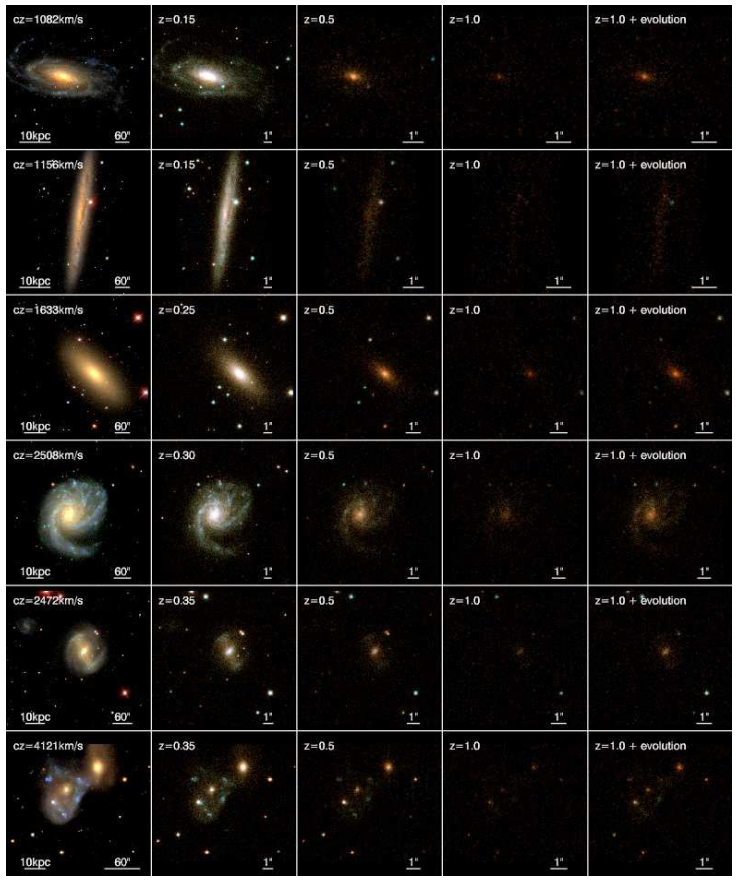
\includegraphics[width=\columnwidth]{Figures/Barden2008.PNG}
    \caption{Artificial redshifting examples as taken from \citet{Barden2008}. From left to right the first four panels in each row show the original SDSS $gri$-colour composite image and the redshifted false colour images at z = 0.15- 0.45, 0.5, 1.0. Apparent scales are indicated in each panel; physical scales are the same in each panel and therefore only marked in the leftmost panel.}
    \label{fig:FERENGI}
\end{figure}

Whilst FERENGI made good progress in the computing side of astronomy, and has been used within further studies since development \citep{Douglas2012}, it comes with its flaws. Some of these have been highlighted in the next section, by the team who worked on AREIA. Mainly, that FERENGI was designed for nearby galaxies in the SDSS, not all galaxies. And, the fact that multiple objects in the same image are not segmented and thus treated as one objects at the same redshift.


\subsubsection{AREIA}
\label{sec:AREIA}

In a more recent study a group made their own implementation of FERENGI and used it for further progress in morphological classification \citep{Ferreira2018}. Their project was named AREIA (Artificial Redshift Effects for IA) and involved changes to the fundamental algorithm of FERENGI, as well as adding their own features. Firstly, FERENGI is limited in only being developed for galaxies in HST surveys. Adaptations were made such that it would work for the EFIGI (Extraction de Formes Idealis\'ees de Galaxies en Imagerie) survey and for instruments beside the HST, which this study was based around. A key difference between this and FERENGI is the approach to dealing with multiple objects in a single image. FERENGI itself does not consider other objects in the image to be separate entities. Everything is treated as one object at the same redshift, when in reality this is likely not the case. This study introduces a procedure to separate out the background objects. The method is outlined in detail in Section 3.4 of \citet{Ferreira2018}. The target galaxy is always centred in the image, making this procedure easier.
Our study involved training a neural network on simulated galaxy images. By simulating our own images, we were able to control a lot of variables such as shape and position. 

\subsection{Deep Learning}
\label{sec:deep_learning}

Deep learning methods have become more frequently used within astronomy over the last decade. In general, these techniques can be classified into two branches - supervised or unsupervised. Supervised learning algorithms take input-output pairs from the user and learn the relationship between the two. Given enough examples, the algorithm can eventually predict an output for a given input. This technique differs to traditional methods as the algorithm creates a model based on the data provided. The data is traditionally fitted to pre-existing models. Unsupervised learning however refers to a broader range of techniques (e.g. dimensionality reduction, detection of outliers, data analysis, etc.). This type of deep learning has the ability to find new relationships within the data since it has been inputted free of labels \citep{Baron2019}. This is an exciting prospect within the world of astronomy.

Completing artificial redshifting procedures using an algorithm for individual galaxies would of course be quite laborious and neither effective nor efficient. However, it has been proposed that the applications of deep learning could be applied to galaxy evolution problems. 
Astrophysicist Marc Huertas-Company has been researching the formation and evolution of galaxies for over a decade.\footnote{Marc Huertas-Company website: \url{https://mhuertascompany.weebly.com/}} His work has been at the centre of this transition to deep learning methods within astronomy. His work has demonstrated that galaxies can be efficiently classified into different evolutionary stages, by using different network configurations, even when no apparent features are visible, as well as to detect and measure substructures within galaxies (i.e. bulges and clumps) \citep{Huertas-Company2021}. Furthermore, using high resolution numerical simulations, rather than simulations which are low in resolution but high in volume or even semi-analytical models, means that realistic observed simulated images can then be generated \citep{Huertas-Company2018}. This means that conclusive statements can then be made since the evolution history of these images is known since they are constructed through simulation, e.g. \citet{Snyder2015}.


\subsubsection{Neural Networks}
\label{sec:neural_networks}

In the most recent decades an emerging approach used for studying galaxy evolution is using Artificial Neural Networks (ANNs), see \citet{Storrie-Lombardi1992}. An artificial neural network can be thought of as a decision making tool. Information is passed through it and the network builds a statistical model around it. The ‘decisions’ it makes are purely made based on probabilities. This reduces the need for human labeling as knowledge is transferred between networks which are trained over different datasets \citep{Sanchez2018}. Neural networks can be used to learn a simplified representation of a galaxy and how they vary, and autoencoders, which are a type of ANN, used to learn efficient data codings in an unsupervised manner (e.g. \citet{Schawinski2018,Glaser2019}), have been used in this way to simulate how a given galaxy would appear if observed at a higher redshift.

The methods featured in FERENGI and AREIA build the statistical models by feeding images of galaxies with ranging redshifts into the network. This is known as a Convolutional Neural Network (CNNs). CNNs are a type of deep learning algorithm used primarily for 2-dimensional image processing within astronomy. CNNs were developed in the 1980s taking inspiration from how neurons within the brain are connected \citep{LeCun1995}. Alike to ANNs, CNNs are still feed-forward networks but within each layer there are restricted connections, so that the following neurons are only connected to a small set of neurons that are in the same region of the input image. Furthermore the weight of the connections are copied across the different neurons effectively giving a convolution, and the size of the network is reduced through subsampling (also known as pooling). These networks require much less pre-processing compared to other classification algorithms and have the ability to learn filters and characteristics. CNNs have been used in a wide range of studies throughout astronomy. For example, the matter distribution in gravitational-lensing systems were previously estimated using maximum likelihood methods which were time and resource consuming. Implementing CNNs into gravitational-lens studies has immensely improved image processing times and allowed for fast, automated calculations of lensing parameters (e.g. \cite{Hezaveh2017}, \cite{Levasseur2017}).
Another benefit of using CNNs are that they can be trained to perform "forward-modelling" transformations, (e.g. \citet{Huertas-Company2018, Perez2019}), which is an extremely efficient process, and can also be reversed in a "backward-modelling" procedure, see \citet{Schawinski2017}. The forward-modelling approach would enable the application of observational effects in a sophisticated manner, where a simulation can be applied for each specific observation. Additionally, in the backward-modelling approach a neural network could be trained to remove observational effects, meaning a system such as this could probabilistically infer what images of high redshift galaxies would look like if they were nearby. 

\section{Method}

\subsection{Simulating Galaxy Images} % Aiden
\label{sec:simulate}

To train our neural network, we need images of galaxies. So, the first step was simulating these images. This gives us basic images of galaxies, unprocessed to account for observational effects. The images also do not contain any other intrinsic spectral information. An example can be seen in Figure \ref{fig:Sersic}. All galaxies generated this way are centred, symmetrical and have a width and height of 60 pixels. Each galaxy in the sample is defined by 5 parameters: ellipticity, effective radius, rotation angle, S\'ersic index and amplitude (surface brightness at the effective radius). For our sample, the galaxies amplitude and S\'ersic index remained constant at 1 and 0.5 respectively. The remaining parameters were chosen from a random distribution. Figure \ref{fig:Sersic2} shows a sample of 25 generated galaxies. This is a good example of how the galaxies can vary in their shape and angle.

\begin{figure}
	\includegraphics[width=\columnwidth]{Sersic-v2.png}
    \caption{A plot of an elliptical S\'ersic galaxy. To give a quantitative perspective to the parameters, this galaxy was produced with an effective radius of 15, ellipticity of 0.3, a rotation angle of $- \frac{\pi}{4}$ and an amplitude of 1.}
    \label{fig:Sersic}
\end{figure}

\begin{figure}
	\includegraphics[width=\columnwidth]{Sersic2-v2.png}
    \caption{A set of S\'ersic galaxies with varying degrees of ellipticity, effective radius and rotation angles. This plot gives an example of how our galaxies vary in shape and brightness prior to applying observational effects. All images are 60 pixels by 60 pixels.}
    \label{fig:Sersic2}
\end{figure}

To simulate a more realistic looking galaxy, we needed to combine images like Figure \ref{fig:Sersic2} with real spectral energy data. SMpy (Section \ref{sec:SMPY}) is a module designed to build a stellar population based on existing models. This module in particular uses the Bruzual and Charlot computational model \citep{Duncan2014,Bruzual2003}. This stellar population model was used to produce a set of SEDs spanning 17 different filters. Figure \ref{fig:SED} shows some of the SEDs. The wavelength range covered is approximately 1,000 \si{\angstrom} to 80,000 \si{\angstrom}. The important data provided was a set of flux values. They correspond to pixel brightness values in our plots, so combining the flux data with the pre-existing S\'ersic images was simple. For the purposes of our application, we kept the redshift range to $0 \leq z \leq 2$. We found that going further than $z = 2$ would result in too many galaxies too dim to observe. Each redshift value in this interval, with an increment of 0.01, provides a unique SED.

\begin{figure}
    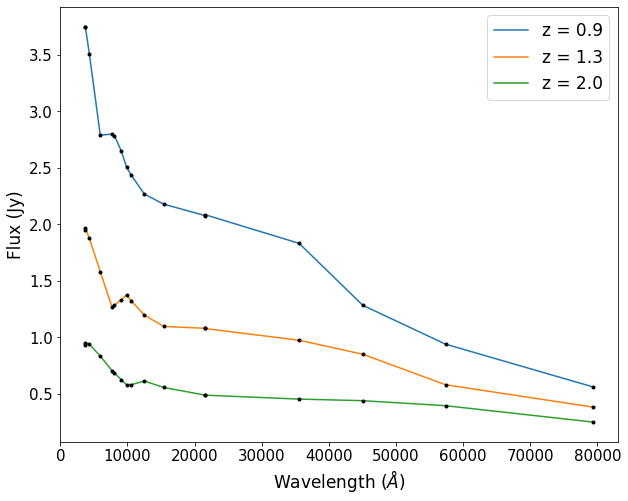
\includegraphics[width=\columnwidth]{Figures/SED.png}
    \caption{A selection of 3 galaxy SEDs within our redshift range of $0 \leq z \leq 2$. These plots include galaxy flux data in 17 different filters spanning roughly 1,000 \si{\angstrom} to 80,000 \si{\angstrom} in wavelength. This corresponds to a range of ultraviolet to low infrared filters.}
    \label{fig:SED}
\end{figure}

The next step was taking a random selection of SEDs and combining them with S\'ersic galaxies, like the one in Figure \ref{fig:Sersic}. The SEDs gave us flux values for a range of redshifts. When combined with the simulated galaxies, we get a random sample of simulated galaxies, across a range of redshifts, observed in 17 different filters (later changed to 9 filters). The top row of Figure \ref{fig:galaxy-SED} is an example of a galaxy viewed at a redshift $z = 1.25$ in all filters. The key difference between the filters is the change in surface brightness from one filter to another. This was the first step in applying observational effects.

The final result of all this is the ability to generate a set of $n$ galaxies, each with a random input and target redshift. Figure \ref{fig:galaxy-SED} shows a comparison of the same galaxy observed at two different redshifts. With a side-by-side comparison, you can clearly see the decrease in surface brightness as redshift increases. This emulates the dimming effect you would otherwise observe from a real, redshifted galaxy.

\begin{figure*}
	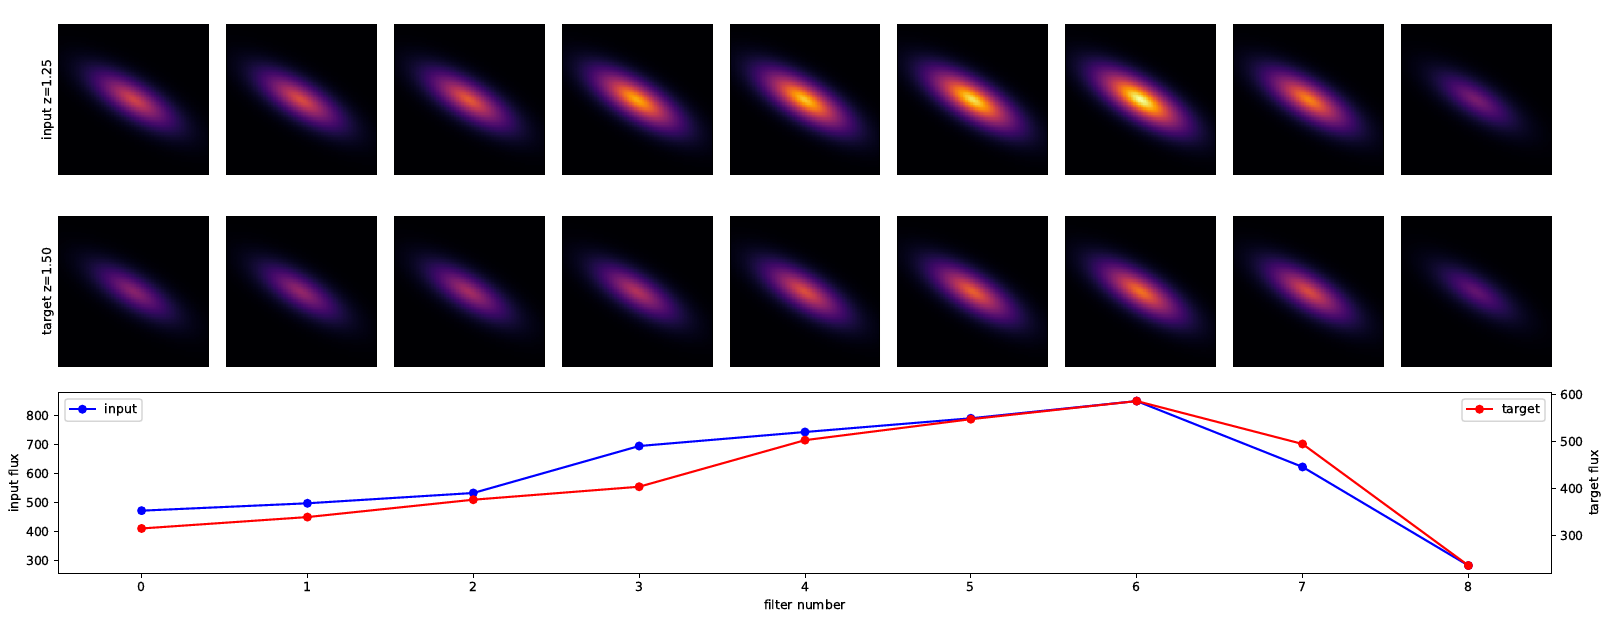
\includegraphics[width=2\columnwidth]{Figures/galaxy-SED-v2.png}
    \caption{A comparison of a galaxy at an input redshift of $z = 1.25$ and a target redshift of $z = 1.5$. Below the galaxy images is a plot comparing the flux of the input and target galaxy across the various filters. The blue line corresponds to the input galaxy and the red line to the target. As mentioned in Section \ref{sec:simulate} the filters range from 1,000 \si{\angstrom} to 80,000 \si{\angstrom}.}
    \label{fig:galaxy-SED}
\end{figure*}

It was later decided to reduce the number of filters included in our sample sets. This would help reduce file sizes, which in turn speeds up the application of observational effects, as well as the neural network training. By reducing the number of filters to 9, we effectively cut the sample data size in half. An important point on this is that we kept the domain of the filters the same. We simply removed some of the filters in the middle of the range. That way, there is no extrapolation required when artificially changing the redshift of a galaxy.

\subsubsection{Stellar populations and Masses with Python (SMpy)} \label{sec:SMPY}
As mentioned previously in Section \ref{sec:simulate}, SMpy (\url{https://github.com/dunkenj/smpy}) was an instrumental tool in creating our simulated galaxies. Before using this tool, we had simple S\'ersic galaxies with no variation in intrinsic galaxy properties. SMpy is a Python module designed for building and processing stellar population modules. When used, this tool produces a wide variety of galaxy properties such as flux and magnitude profiles for a simulated stellar population. The important thing we wanted to extract was the galaxy SEDs. The galaxy SEDs contain a lot of information, including: star formation history, cosmological age, metallicities and dust contents. The spectral data produced is based on an existing population model \citet{Bruzual2003}. Bruzual and Charlot is a model used for computing the spectral evolution of stellar populations across a range of ages. The data produced is based on typical galaxies from the Early Data Release (EDR) and the SDSS.

\subsubsection{Simulating Complex Galaxy Images} \label{sec:complex}
After running many tests on our network with the simulated galaxy images (Section \ref{sec:increasing-redshift} \& \ref{sec:decreasing-redshift}) we decided to generate galaxies with more intricacies to further challenge the networks ability to make reconstructions. We had two approaches to this idea: overlaying two sets of S\'ersic galaxies and generating asymmetric S\'ersic galaxies.

Up to this point, our galaxies were fairly simple shapes - a disk with no additional structures. A more realistic galaxy would be observed to have a central bulge with a surrounding disk. Obviously real galaxies can have far more complex features than this, such as spiral arms. But, this was a step in the right direction. In order to generate galaxies with a bulge and disk, we first generated two sets of S\'ersic galaxies. One set was constrained such that the shape would remain small and circular, like a bulge. The second set was constrained to be larger and elliptical. By summing the sets together we obtained a set of galaxies with more variation in shape. The result of this process can be seen in Figure \ref{fig:complex-galaxy}.

\begin{figure}
	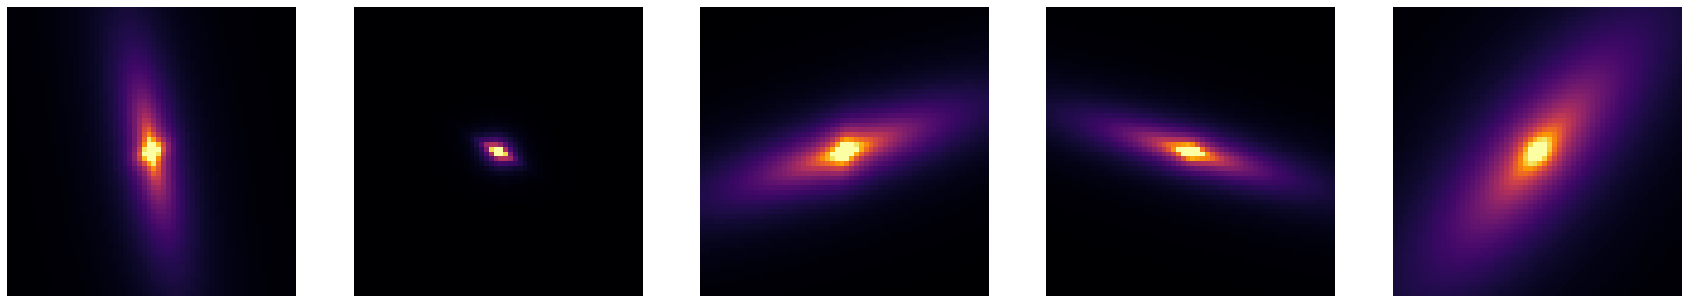
\includegraphics[width=\columnwidth]{Figures/complex-galaxy-v2.png}
    \caption{A set of complex S\'ersic galaxies - all containing a central bulge and surrounding disk. This increases the variation in shape available to us, allowing us to further challenge the networks ability to make reconstructions.}
    \label{fig:complex-galaxy}
\end{figure}

All galaxies generated in our original sample set were perfectly symmetrical about the axis of the galaxy, but in reality galaxies are not always symmetric. Some additional parameters were introduced to allow for asymmetry in the sample. This being the angle of asymmetry and the strength of the asymmetry. The variation this change added to our sample can be seen in Figure \ref{fig:asym-galaxy}. Unfortunately, we were not able to run these galaxies through the network due to time constraints.

\begin{figure}
	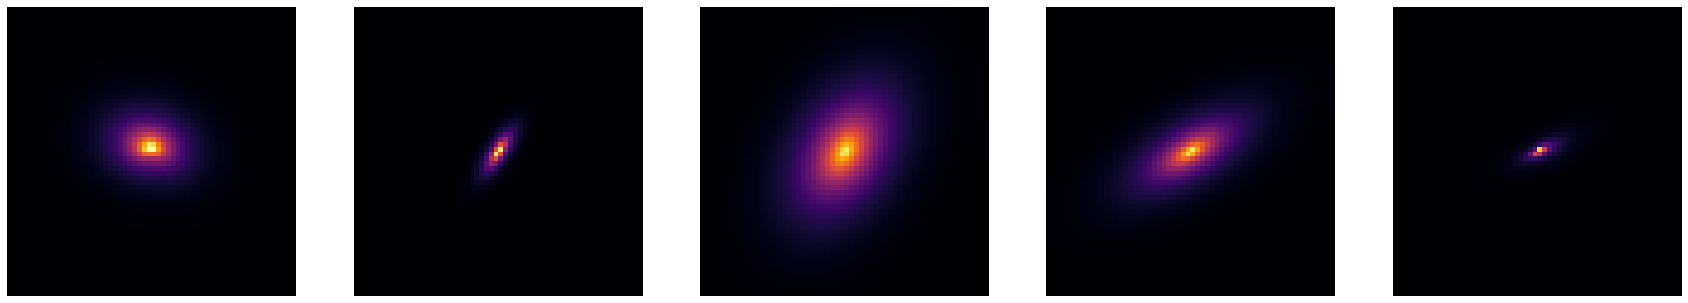
\includegraphics[width=\columnwidth]{Figures/asym-galaxy-v2.png}
    \caption{A set of asymmetric S\'ersic galaxies. These galaxies have the addition of extra, randomly chosen parameters - the angle of asymmetry and strength of asymmetry.}
    \label{fig:asym-galaxy}
\end{figure}

\subsection{Applying Observational Effects} % Liz
\label{sec:observe}
Up to this point, we have sets of galaxy images that have some observational effects, such as dimming, but are still lacking in others. The images obtained thus far are suitable to begin training with. The neural network can be trained to reconstruct a galaxy at a target redshift, given the same galaxy at an input images. To begin with, the input redshift will always be lower than the target. Following the same procedure used in \citet{Barden2008}, further observational effects were applied to the simulated galaxy images. Each effect was applied in its own function, allowing the possibility to select which effects we wanted to apply for different runs of the network later on. The AREIA \citet{Ferreira2018} code served as a starting point for this section of code (\url{https://github.com/astroferreira/areia}).

\subsubsection{Rebinning}
\label{sec:rebinning} 
In order to better mimic the observation of the input galaxy at a higher target redshift, the images need to be rebinned. In doing so we wanted to preserve the size of the images, whilst changing the apparent size of the galaxies. When converting between different values of redshift the angular size $a$ changes as,
\begin{equation}
\label{ang_size}
\frac{a_o}{a_i} = \frac{d_i / (1 + z_i)^2}{d_o / (1 + z_o)^2}
\end{equation}
where $d_i$ and $d_o$ are the input and output luminosity distance respectively. This relation was used as a scale factor to appropriately re-bin the images through Python's zoom function. However the use of this function alone does not preserve the size of the images. As a result, when transforming from low to high redshift, the overall image size would decrease. In order to keep the 60 by 60 pixel size constant, the images were subsequently resized using broadcasting and interpolation techniques (method detailed in \url{https://gist.github.com/bamford/4ccc4da519bba5216f58d12070865fc3#file-test_rebinning-ipynb}). This method interpolated pixels from the original images and created a re-scaled grid of values, but with a constant number of pixels. It was important to ensure the image size remained constant for use in training the neural network later on. The second row of Figure \ref{fig:obs_eff} demonstrates the outcome of this effect. Figure \ref{fig:obs_eff} also demonstrates all other observational effects being applied to the example simulated galaxy image.

\subsubsection{Point Spread Function (PSF)}
\label{sec:psf}
When observing a galaxy through a telescope, there are certain observational effects caused by the telescope itself. Namely, the optics of the instrument. As well as this, turbulence in the Earth's atmosphere also contributes to the PSF. An object that would otherwise be observed as a point source is observed as "blurry". By applying a PSF to our set of galaxy images, we can emulate such an effect. In turn, this will train the network to account for these types of effects. 

Just like the galaxies, the PSF was artificially created by us. We chose to use a uniform Gaussian kernel with a seeing of $3.5$. The seeing is the full width half maximum of the kernel. This kernel was convolved with the simulated galaxy images to produce an image like that seen on the third row of Figure \ref{fig:obs_eff}. The same uniform kernel was applied to all images in the sample.

\begin{figure}
	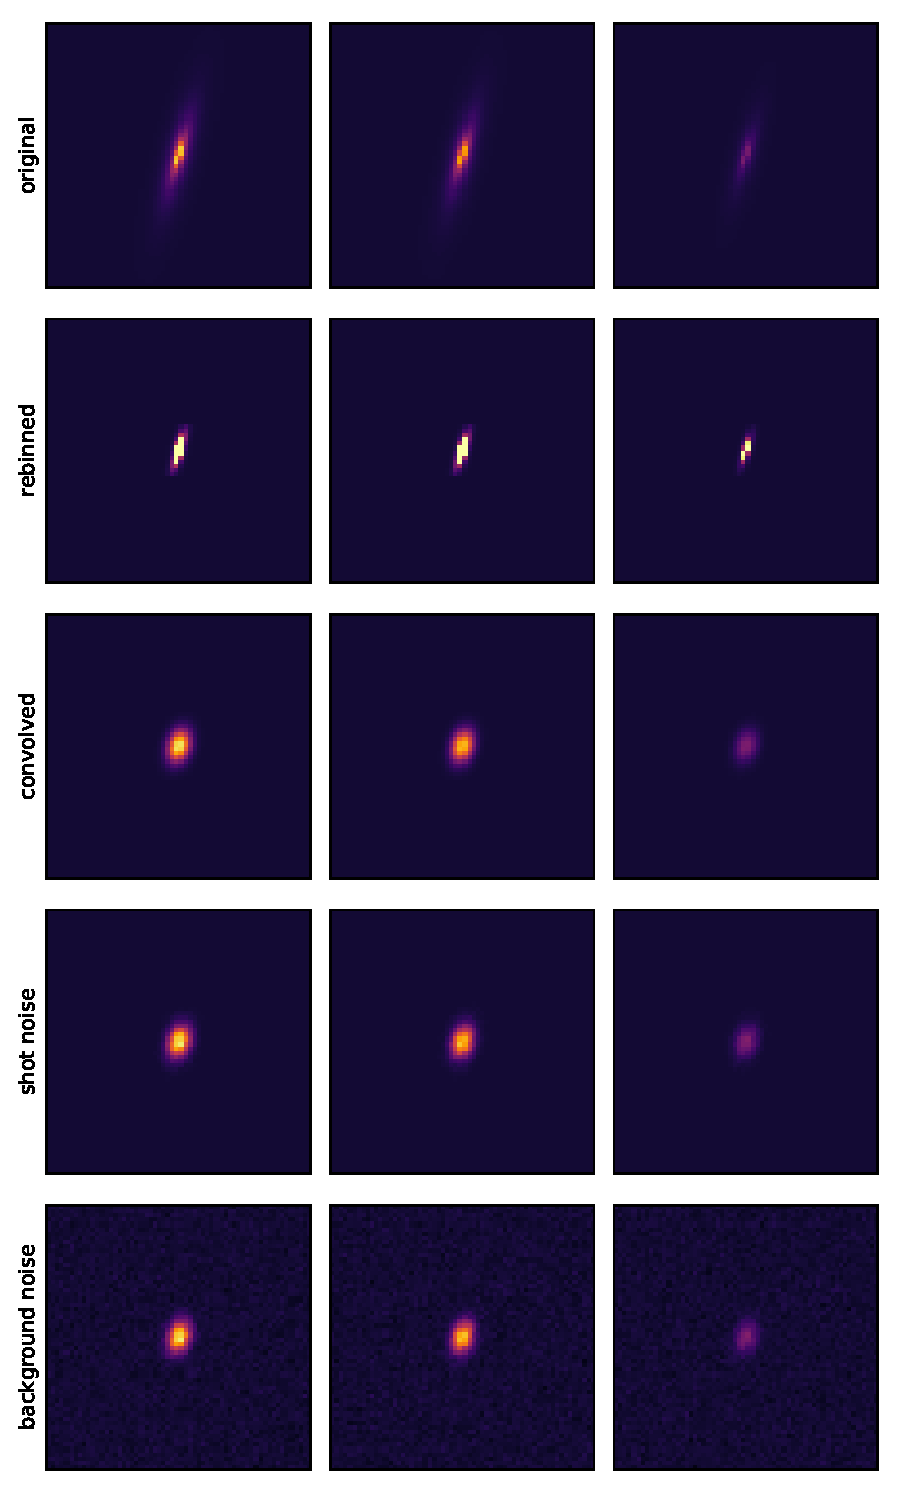
\includegraphics[width=\columnwidth]{Figures/obs_eff_2.pdf}
    \caption{An example of each observational effect being applied to a randomly selected galaxy from the training set. The top row indicates the original image in a three different filters. The second row demonstrates the same galaxy after rebinning and the third row after convolving the image with the PSF. Lastly, the fourth and fifth rows show the images after adding shot noise and background noise, respectively. Though each effect may be subtle, as a group they dramatically improve the realism of our simulated galaxies. These effects are necessary as we want our network to be able to accurately process actual images in the future. Therefore, training with simulated images which are as close to real images as possible is important.}
    \label{fig:obs_eff}
\end{figure}

\subsubsection{Noise}
\label{sec:noise(all)}
Adding noise is an instrumental step in outputting realistic galaxy images. There are two primary sources of noise when observing distant galaxies; shot noise from the galaxies themselves, and background noise which has several contributing factors.

\paragraph{Shot Noise} \label{sec:shot}
Shot noise originates from fluctuations in the light arriving from the observed galaxy. This is quantified by a variation in the number of photon counts detected by each pixel that are arriving from the source. To model this variance, a simple Poisson distribution was added to the images. This distribution was applied to model the shot noise as the number of fluctuations in the light arriving from the object itself is relatively low. The fourth row of Figure \ref{fig:obs_eff} shows the application of shot noise. 

\paragraph{Background Noise} \label{sec:background}
The second type of noise that must be considered is background noise. This has several sources. Firstly, shot noise from the sky, also known as sky noise. This is caused by the randomness of the detection of photons in the Earth's atmosphere. Sky noise can usually be accounted for when observing astronomical objects by simply subtracting a reading of blank sky from the images. In addition to sky noise, there is also dark noise and read out noise. Dark noise occurs as a result of electrons in the detector which appear randomly from thermal noise. Lastly, read out noise can appear through the amplification of observed signals. 
Each of these sources contribute to the background noise and are usually individually measured for removal. However in this instance we wished to add the effects of background noise in order to obtain a more life-like image. Like the shot noise, the background noise can be modelled as a distribution function. In this case a Gaussian distribution was added to images as the number of these random photon counts is much larger due to numerous sources. The fifth row of Figure \ref{fig:obs_eff} shows the background noise being applied to an example galaxy.



\subsection{Building the Network}
\label{sec:network}

The neural network created is a CVAE, which consists of an encoder, decoder and loss function. The full script for the network can be found at \url{https://github.com/aidenrolfe/ARG} and was originally based on the existing Keras Variational Autoencoder (VAE) example (\url{https://keras.io/examples/generative/vae/}). The final architecture of the network is based on input images of a 60 by 60 size with 9 channels (which in this case is the number of filters the galaxy is observed in). The image data is initially passed through an encoder consisting of 4 convolutional layers of a 3 by 3 kernel size and a dense layer with an output shape of 64, which produces a latent space of 20 dimensions. The data is then passed through the decoder which contains a dense layer with a 7*7*64 output, followed by a further 4 convolutional layers of a 3 by 3 kernel size. This is finally followed by the loss function which regularises the model, in which beta is set to be 1 as this value was found to not negatively effect the reconstruction loss.

The earliest examples of the network however, were built and trained using MNIST data with a 28 by 28 image size. This is because the simulated galaxies, redshifted galaxies and artificial observational effects (as described in Section \ref{sec:simulate} and \ref{sec:observe}) were being created simultaneously, so were not initially ready to be used to train the network from the outset.

\subsubsection{MNIST Dataset}
\label{sec:network_MNIST}

Once the initial network was built and worked well simulating MNIST data, an approach was then made to ‘de-noise’ the MNIST digits. To do this the dataset was imported and then random uniform noise was added with the resultant images then fed to the network. Initially the network could replicate the noisy images fairly well, so then it was developed to effectively recreate the digits with no noise, as shown in Figure \ref{fig:MNIST}. 

\begin{figure}
\begin{subfigure}[b]{\columnwidth}
	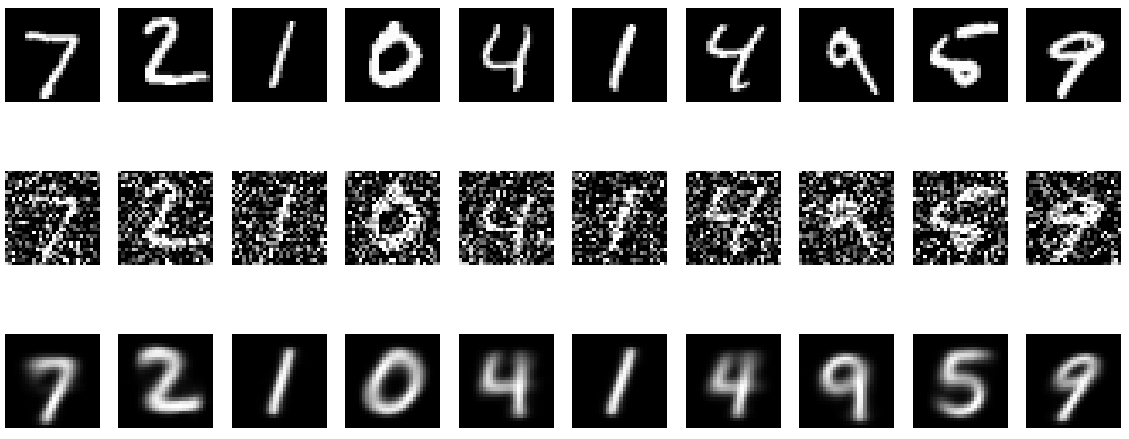
\includegraphics[width=\columnwidth]{Figures/mnist_blackwhite.png}
    \caption{Original black and white MNIST digits. Whilst the reconstructions are slightly blurry in comparison to the target, the network has still de-noised and reconstructed the shape very well.}
    \label{fig:MNIST}
    \end{subfigure}
    
 \begin{subfigure}[b]{\columnwidth}
	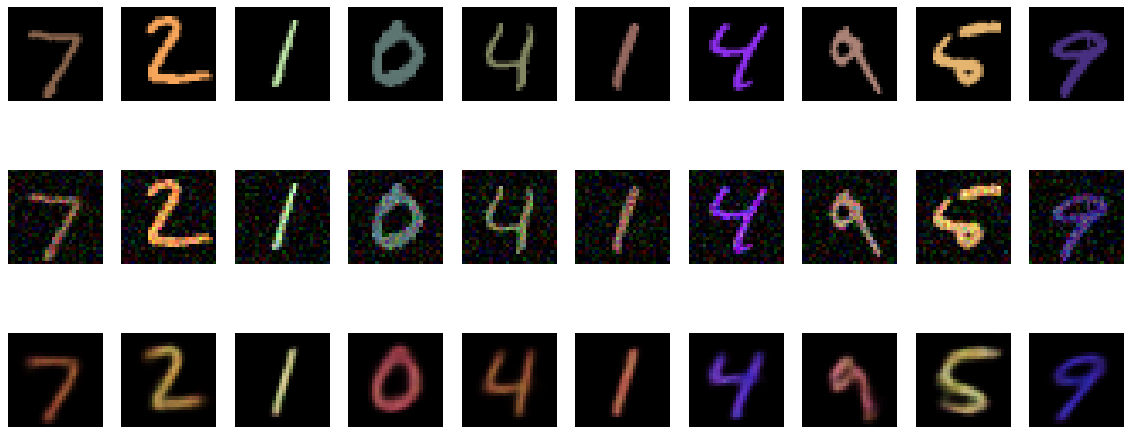
\includegraphics[width=\columnwidth]{Figures/mnist_colour.png}
    \caption{Multi-channel coloured MNIST digits. Whilst the colour of the reconstructions is somewhat off, the network has still de-noised and reconstructed the shape of the digits very well.}
    \label{fig:colour_MNIST}
    \end{subfigure}
    
        \caption{The first row shows the original MNIST digits which were the target image for the network. The second row shows these digits with added random uniform noise which were the input image for the network. The third row shows the digits reconstructed by the network in which the input images have been successfully de-noised.}
    \label{MNISTPlots}
\end{figure}

In this simplistic example the 9 digit classes were given as a condition in the encoder as this meant that the conditions could then be processed by a couple of fully-connected layers and one non-linearity in producing the latent encoding, but avoided complications that would arise if they were added in even earlier. This allowed the network to learn the basic features but not depend heavily on the labels, allowing the encoding process to be a more efficient representation of each class. The conditions were then included again in the decoder as this meant that the latent encoding did not need to include the condition, so could be more efficient, and also that if the decoder is then used alone the condition can be specified. These conditions were categorical, rather than a continuum, thus in this case it was more appropriate to use a set of class inputs, giving the probability that the label belongs to each class. A series of if/else loops were added in so that the application of these conditions was optional, thus the effect this had on the training in latent space could then be viewed, where when the condition was applied the digit classes were more distinct in the latent space plots as shown in Figure \ref{fig:if/else plots}.

\begin{figure}
    \begin{subfigure}[b]{\columnwidth}
        \centering
	    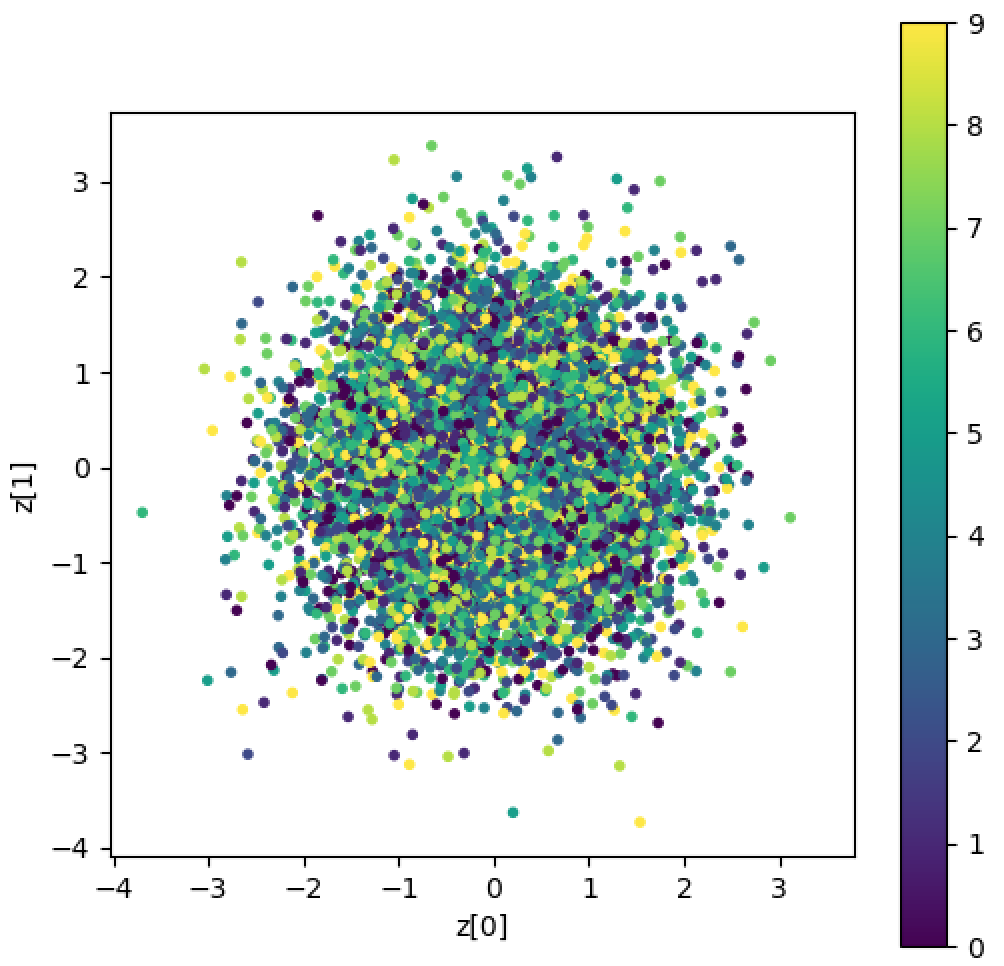
\includegraphics[width=\columnwidth]{Figure_29a.png}
        \caption{Digit class condition applied resulting in less structure in latent space training.}
        \label{fig:cond}
    \end{subfigure}
    
    \begin{subfigure}[b]{\columnwidth}
        \centering
	    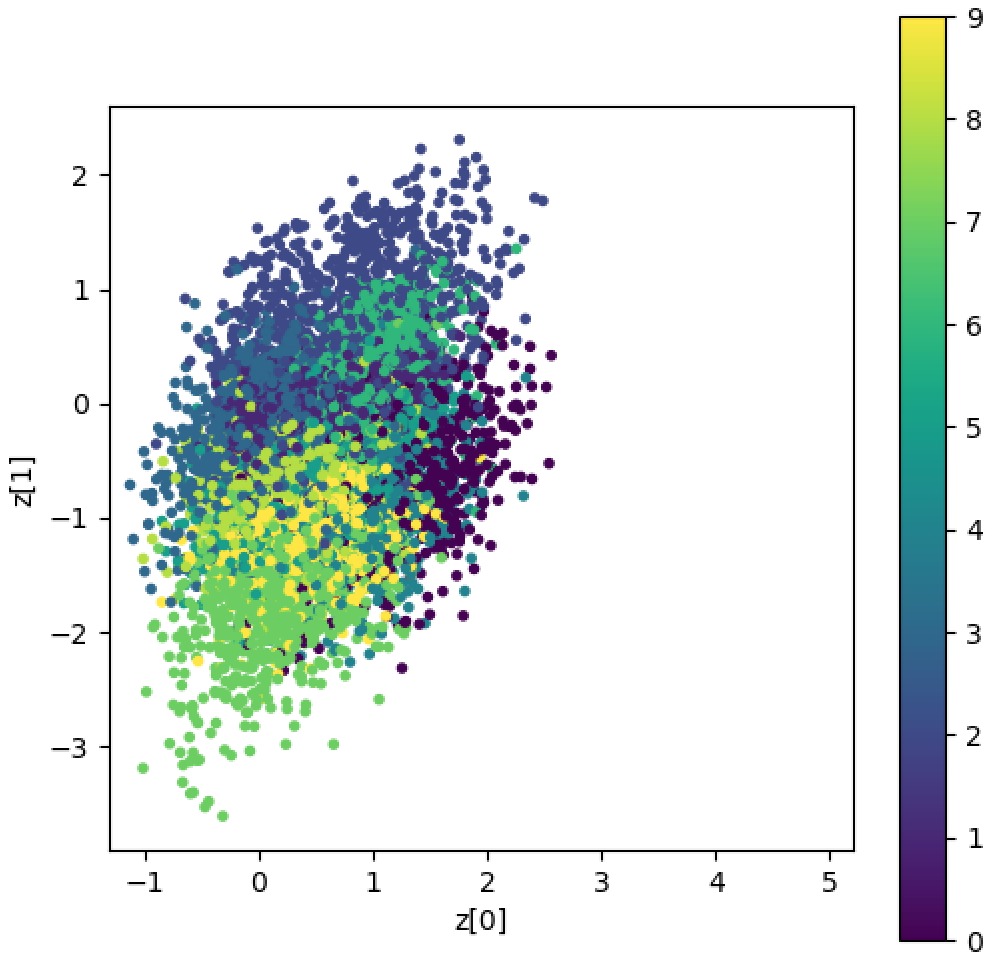
\includegraphics[width=\columnwidth]{Figure_29b.png}
        \caption{Digit class condition not applied resulting in structure in the latent space training where it can be viewed that each digit class tends to be grouped together.}
        \label{fig:no cond}
    \end{subfigure}

    \caption{2D plot of digit classes in latent space where the colour bar indicates the digit class of the of the points.}
    \label{fig:if/else plots}
\end{figure}

The MNIST digit data was then edited so that it was ‘multi-channel', in preparation for using the network with images of simulated galaxies. This was done by duplicating single channel content $c$ times along the final axis, where the original input data previously had a shape of $(n, w, h, 1)$ it then became $(n, w, h, c)$. The most elegant solution posed to this was to use array broadcasting, where when 2 arrays of different shapes are operated on, one is broadcasted over the other. This worked successfully so noise was then added to these coloured MNIST digits, and the network was then successfully trained to repeat the previous process in which it then ‘de-noised’ these digits, as shown in Figure \ref{fig:colour_MNIST}. At this point an early stopping callback was also added in so that if there was no improvement to the validation loss after 15 epochs then training ceased \citep{Raskutti2013}.

\subsubsection{Simulated Galaxies Dataset}
\label{sec: network_gal}

As all previous tests were fairly successful, the network then began to be trained using the initial simulated galaxy data without the artificial observational effects applied. The simulated galaxy and redshift data were created using the method in Section \ref{sec:simulate} and then imported. As the aim of this initial experiment was just to test the how well the simulated galaxies could be reproduced without observational effects applied, the target and input redshift arrays contained only one number. Thus, each redshift array was duplicated to be the same size as the galaxy target and input data arrays, and then finally these redshift arrays were transposed together. The simulated galaxy data as well as redshift data was then shuffled and split with 20\% of the data allotted to a test subset, and the remaining 80\% to the train subset. The number of conditions within the encoder was then changed to 2 since there is only an input and target redshift now instead of 9 digit classes. These initial experiments were run using smaller sets of training images ($\sim$1,000), as this had the most reasonable run time to reconstruction quality ratio, and reconstructions that were created for the most part seemed to work well. However, loss was still quite high, so to improve this the final convolutional ‘sigmoid’ activation layer in the decoder was removed, as the output could not be assumed to be between 0 and 1 as was the case for the MNIST digits. The galaxy images have very different overall normalisation (although not far off a standard deviation of 1) in comparison and are more all over the place, depending on the redshift. Running the network after implementing these changes resulted in losses of NaN, so then want on to rectify this by investigating normalising the galaxies individually. This may seem like the removal of useful information, but this information is only necessary to interpret and reproduce the noise correctly (and noisy images were not yet being used) and also the normalisation values could be added into the network as a condition alongside redshifts. Therefore the input of this significantly lowered the loss and made for very good reconstructions as shown in Figure \ref{fig:gal_1}. 

\begin{figure*}
	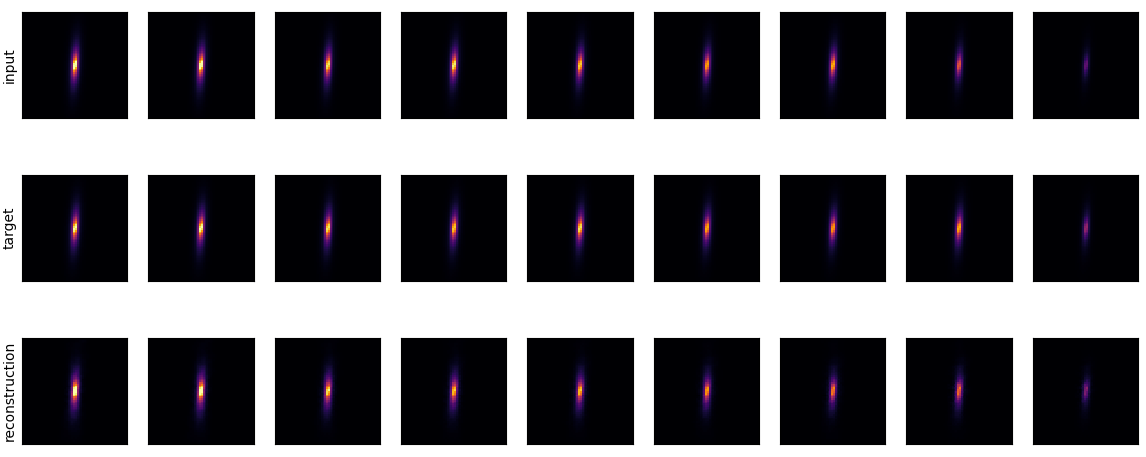
\includegraphics[width=1.85\columnwidth]{Figure_62a.png}
    \caption{First row shows input galaxy with a low redshift of 1.0  in 9 different filters. The second row shows the galaxy at the target high redshift of 1.6. The third row shows the reconstructions made by the network, which match up with the second target row extremely well.}
    \label{fig:gal_1}
\end{figure*}

Since the difference between the target and reconstruction images was marginal and not quantifiable by eye, the plotting of a residual image was then introduced to better quantify the quality of the reconstructions. This was calculated by plotting the difference between the target and reconstruction images. The residual value was then shrunk by a factor of 10 so that the more subtle differences between the target and reconstruction images are able to be seen. Whilst these residuals then gave a good visual aid as to the level of error in the reconstructions they were still not quantifiable. Therefore, to calculate an approximate value for the error the residual images were divided by the target images to get a fractional error per pixel. These values were then multiplied by 100 to give the percentage error per pixel as shown in \ref{fig:errorplot}. In order to get a percentage error for the whole image these percentage errors per pixel were then averaged across an area enclosed by a circle surrounding the galaxy centre, for which the radius was selected to encompass the majority of residuals surrounding the centre.

\begin{figure}
	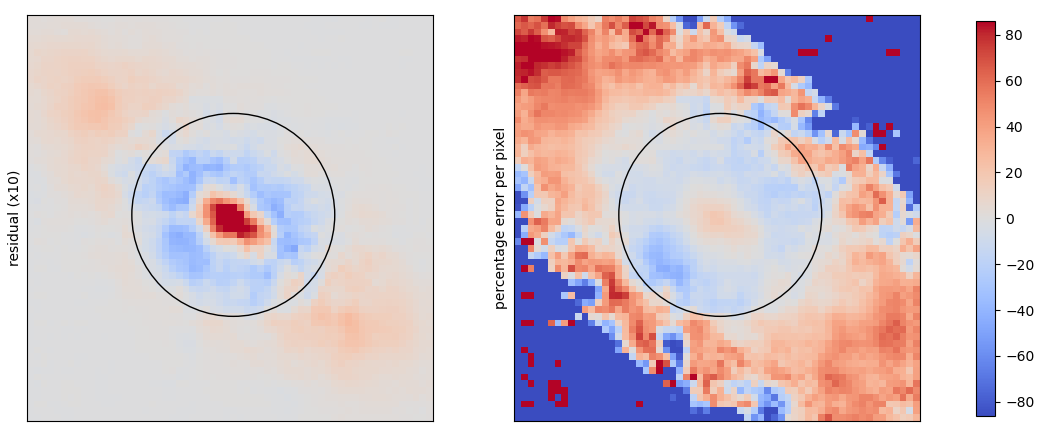
\includegraphics[width=\columnwidth]{Figures/percetage_error.png}
    \caption{Residual and percentage error per pixel between the reconstruction and target image for the fifth filter of complex galaxy experiment as shown in Figure \ref{fig:complex-noisy-high-standard-low}. The colour bar indicates the percentage error per pixel on the right plot, where in this case within the circle the average error per pixel is 10\%.}
    \label{fig:errorplot}
\end{figure}

Then started to experiment with the introduction of artificial observational effects as described in Section \ref{sec:observe} and the reconstruction of these ‘noisy’ images. The resultant was that the network was able to create fairly good reconstructions of artificially redshifted ‘noisy' galaxies, but with very high losses. High losses in this case are to be expected, since the network cannot learn the random noise that each galaxy image contains. Therefore, since the reconstructions were of a high quality and the residuals were minimal the network was attributed to be successful and eligible for future more complex experiments.

For all models created plots of the model loss on the training and validation set were also created, as shown in Figure \ref{fig:model_loss}. This helped to visualise model performance, with the train learning curve giving an idea of how well the model is training and the validation learning curve giving an idea of how well the model is generalizing. The plotting of both of these lines also helps to identify whether the model is underfitting, overfitting, or a good fit. Figure \ref{fig:model_loss} was created in the experiment described in Section \ref{sec:standard-test} and shows both lines decreasing to a point of stability with a minimal gap between them at which point training stops indicating a good fit. An underfit model is indicated by a training loss line that is still decreasing when the training stops, and an overfit line is indicated the validation loss decreasing to a point and then increasing again before training has ceased.

\begin{figure}
	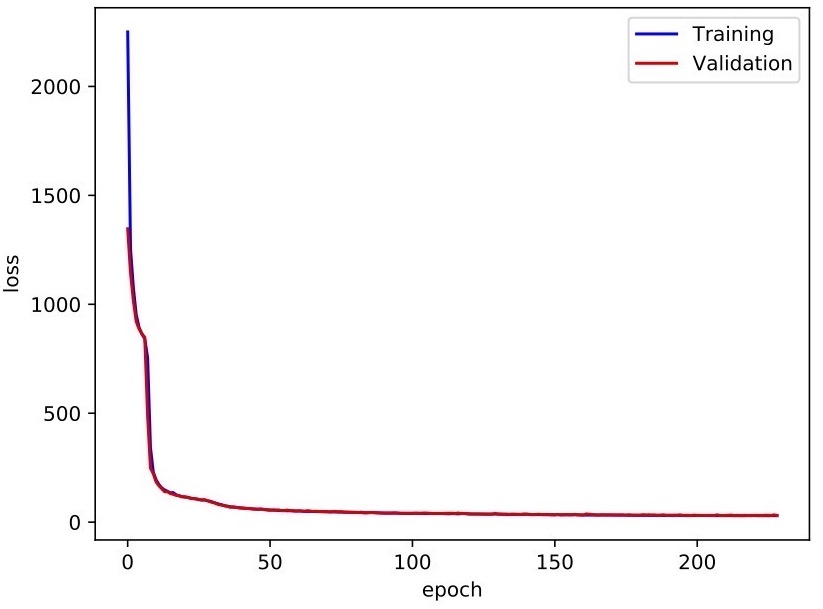
\includegraphics[width=\columnwidth]{Figures/model_loss.jpg}
    \caption{Plot of model loss on the training and validation sets in comparison to epoch number during the training of the model created described in Section \ref{sec:standard-test}. The convergence and simultaneous levelling off of the lines indicates a good fit.}
    \label{fig:model_loss}
\end{figure}

In addition to the plots of model loss, a t-SNE of the latent space for each model was also created. A t-SNE plot is a way of projecting the multi-dimensional latent space down into 2 dimensions in a way that tries to keep neighbouring regions together, as described in \citet{Maaten2008}. The production of this plot, as shown in Figure \ref{fig:t-SNE}, was useful in checking whether the model was training correctly. Since the type of autoencoder used was a CVAE this meant that there should not be any noticeable structure as in Figure \ref{fig:no cond} and there should be a good spread of data points. Galaxies that have a similar appearance or similar SEDs would be expected to be grouped together within the latent space, which can be seen in Figure \ref{fig:t-SNE}.

\begin{figure*}
	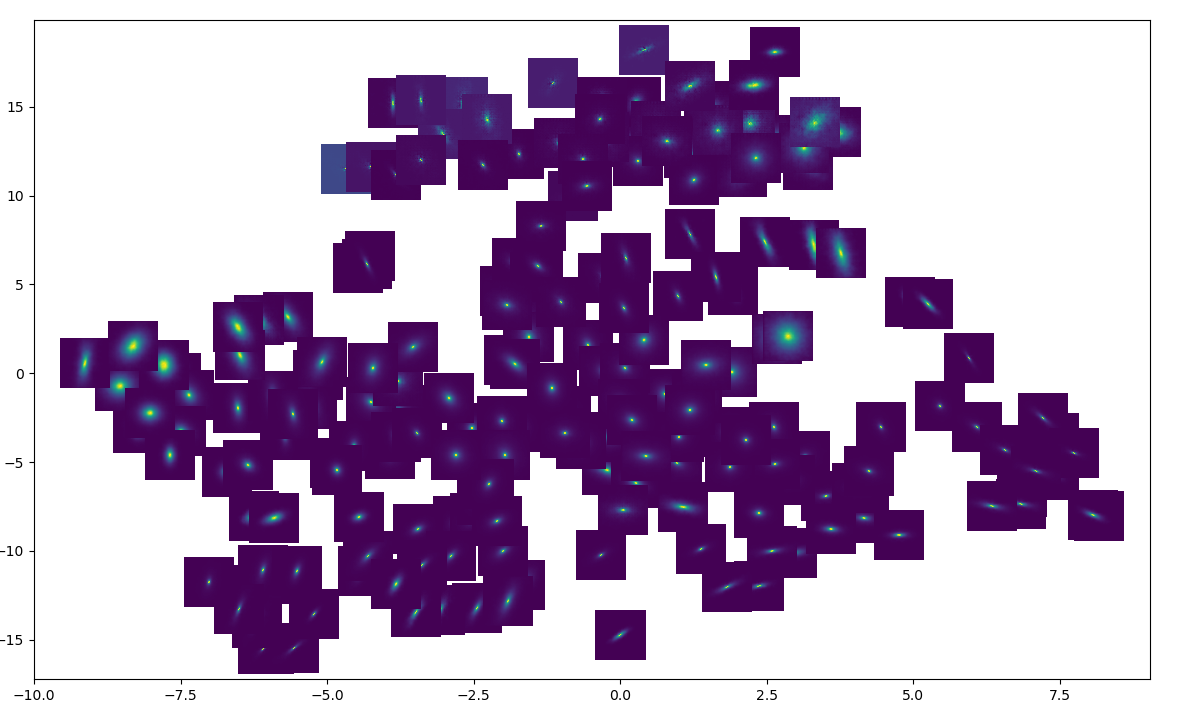
\includegraphics[width=2\columnwidth]{Figures/t_SNE.png}
    \caption{Plot of the latent space in which 20 latent dimensions have been projected down into 2 dimensions. This plot was created using 2500 training images in the creation of the model described in Section \ref{sec:standard-test}. There is a good spread of data points, and galaxies with similar SEDs and appearances are grouped together, indicating successful training for VAE.}
    \label{fig:t-SNE}
\end{figure*} 

A Gaussian noise layer with a standard deviation of 0.2 was added to the encoder in order to regularise the model and reduce the possibility of overfitting. It does this by adding noise to the input images directly which prevents the model from learning the dataset ‘too well', so that it can be used to make effective predictions for new images.

Finally, the plotting of the SEDs to compare the input, target and reconstruction fluxes was added. This allows for a more quantifiable comparison as to the quality of the reconstructions. Whilst the error on the reconstruction SED is not able to plotted as the network does not output a value for this uncertainty, the errors on the SEDs for target and input flux where the galaxies have been ‘observed' and observational effects have been added is able to be shown. This error is calculated by assuming Poisson errors on each count, meaning that the error on the flux is $\sqrt{n}$ where $n$ is the value of the flux at that point.

\section{Results}
\label{sec:results}
\textit{All tests on the VAE were run with a sample of 10,000 randomly generated galaxies, 20 latent dimensions, a beta of 1 and a patience of 15 (meaning if there was no improvement to the validation loss after 15 epochs then training would cease).}

\subsection{Increasing Redshift} \label{sec:increasing-redshift}
\subsubsection{Standard Galaxies} \label{sec:standard-test}
The first step in training the network involved using our simulated images, without some of the observational effects applied (rebinning, PSF, shot noise and background noise). With a set of 10,000 galaxy images, we trained the network to reconstruct each galaxy at a higher redshift, given that same galaxy at a lower redshift. All runs were performed with the consistent split of 80\% for training and 20\% for testing. Following this, we ran another test with the same galaxies, but where the network reconstructs galaxies at a lower redshift, given the higher redshift image (Section \ref{sec:standard-test2}). Thus, reversing the process. In both cases, the network was able to reconstruct the target galaxy very well.

Figure \ref{fig:standard-low-high} gives an example of how the network deals with reconstructing a higher redshift galaxy, given the same galaxy at a lower redshift. The reconstructions made by the network were very accurate, which is reflected by how small the residuals are. From this we can see that the network has no trouble reconstructing the dimming effect that occurs when going from a low redshift to one higher. Moreover, the network is reconstructing the shape and surface brightness of the target galaxy impressively well.

\begin{figure*}
    \begin{subfigure}[b]{2\columnwidth}
        \centering
	    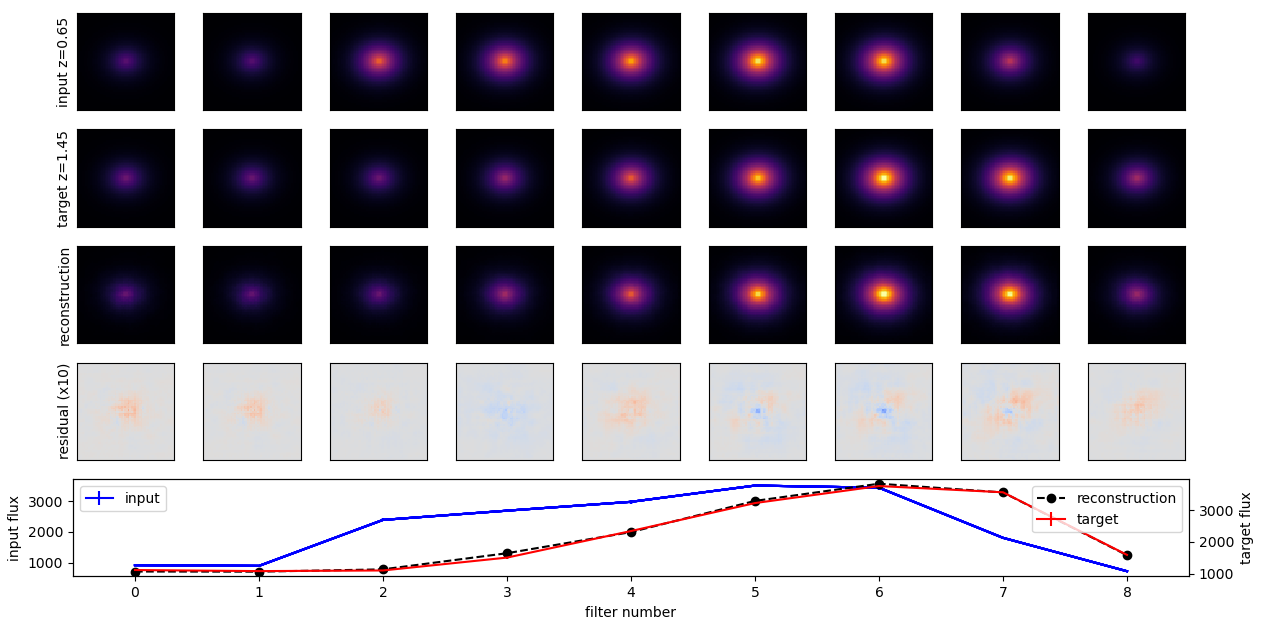
\includegraphics[width=\columnwidth]{Figures/standard-low-high.png}
        \caption{Redshifting a simple galaxy image with no observational effects applied. Residuals are minimal in this case and the reconstruction SED falls within the error bars of the target SED.}
        \label{fig:standard-low-high}
    \end{subfigure}
    
    \begin{subfigure}[b]{2\columnwidth}
        \centering
	    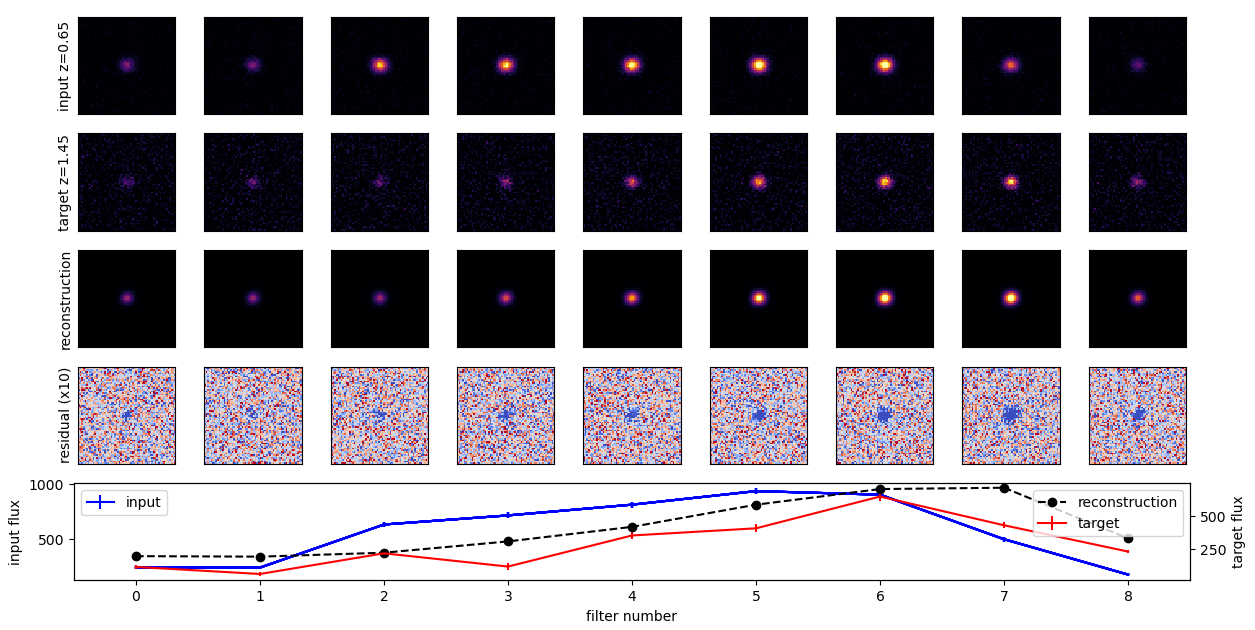
\includegraphics[width=\columnwidth]{Figures/noisy-low-high.png}
        \caption{Redshifting a simple galaxy image with observational effects applied. Residuals are high due to the random noise within the image and the reconstruction SED does not match up with the target SED for most filters.}
        \label{fig:noisy-low-high}
    \end{subfigure}

    \caption{This galaxy has a low input redshift of 0.65 and a high target redshift of 1.45. The first row is the input redshift and the second row is the target redshift. The third row is the image reconstructions that the trained model has produced with the fourth row showing the residuals between the target and reconstructions. The plot on the fifth row shows the SEDs for the input, target and reconstruction images. The input and target SEDs have error bars correlating to the number of Poisson errors on each count.}
    \label{fig:simple galaxy results plots redshifting}
\end{figure*}

\subsubsection{Observed Galaxies} \label{sec:observed-test}
After putting the galaxies through the artificial redshifting process, outlined in Section \ref{sec:observe}, we trained the network to reconstruct the galaxies, as well as the added effects at different redshifts. This is where we found the limitation of the network. Specifically, the way the network reconstructs noise (Section \ref{sec:shot} and \ref{sec:background}). Despite this, the network's ability to reconstruct the galaxies shape and size is retained.

Similar to the tests in Section \ref{sec:standard-test}, we started with a lower redshift input galaxy and a higher redshift target galaxy. The residuals consist mostly of background and shot noise. It may seem like the reconstructions are overall poor after seeing this, however, looking at the reconstruction itself, the galaxies are still reconstructed well; all that is missing is the noise. Figure \ref{fig:noisy-low-high} shows an example of a particularly noisy galaxy. The residual plot on the bottom row shows small inaccuracies in the reconstruction of the galaxy, but is mostly dominated by noise.

\begin{figure*}

    \begin{subfigure}[b]{2\columnwidth}
        \centering
	    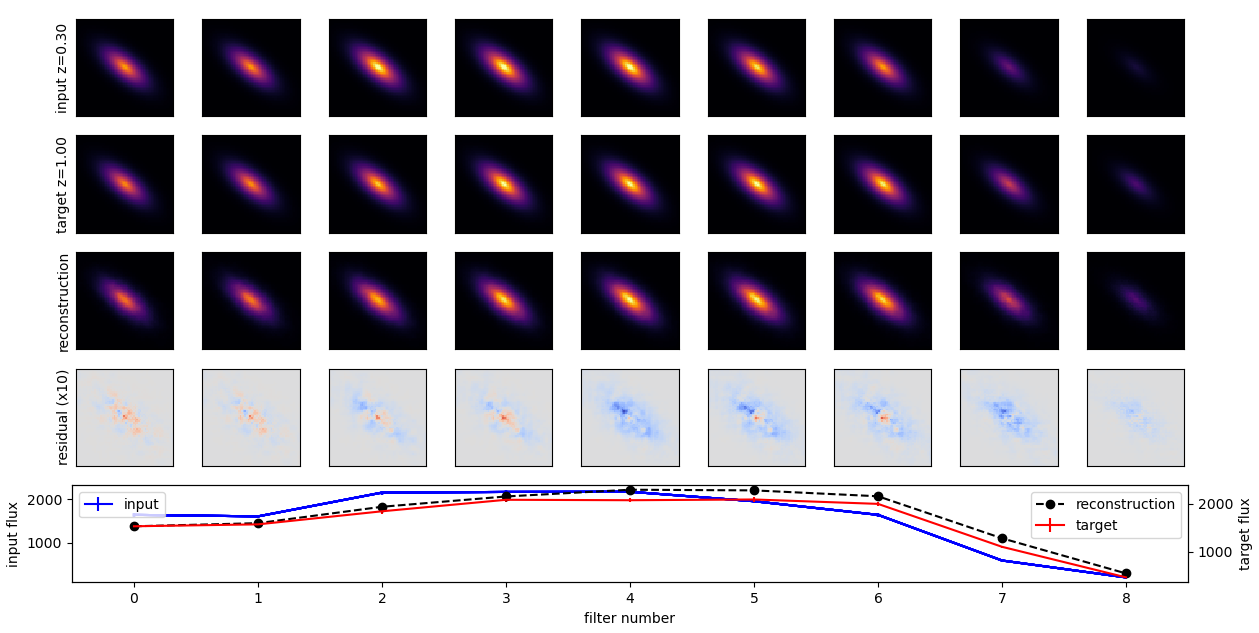
\includegraphics[width=\columnwidth]{Figures/bd-standard-low-high.png}
        \caption{Redshifting a complex galaxy with no observational effect applied. The residuals are fairly minimal and the reconstruction SED falls within the error bar range of the target SED for most filters.}
        \label{fig:complex-standard-low-high}
    \end{subfigure}
    
    \begin{subfigure}[b]{2\columnwidth}
        \centering
	    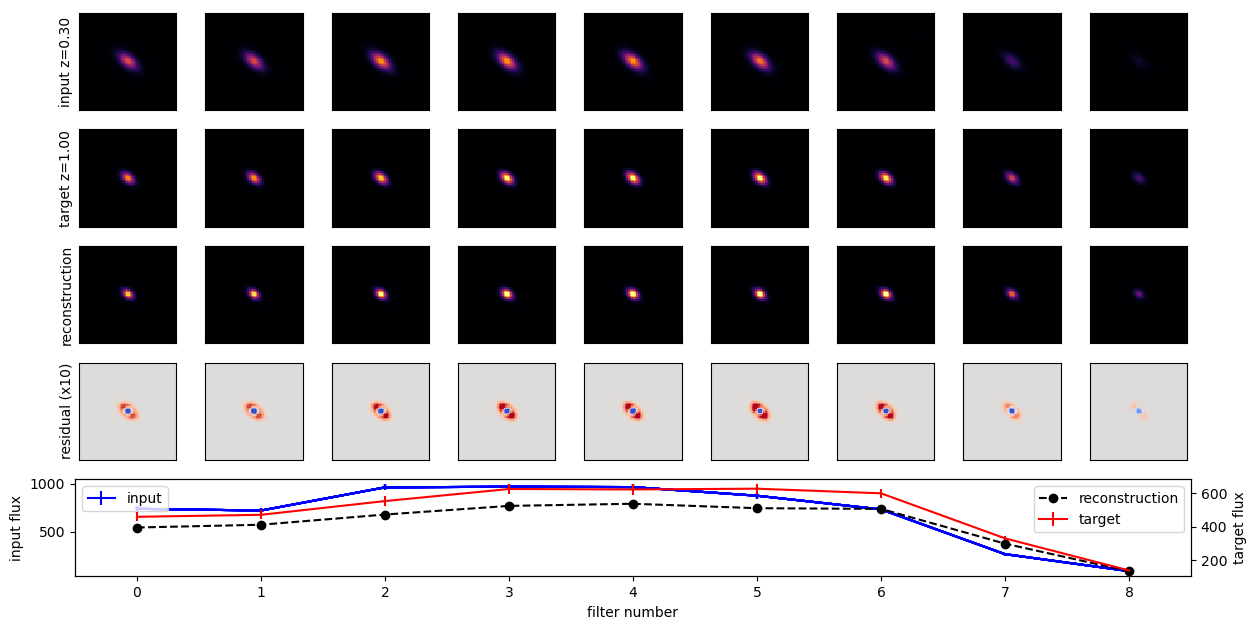
\includegraphics[width=\columnwidth]{Figures/bd-noisy-low-high.png}
        \caption{Redshifting and de-noising a complex image with observational effects applied. Residuals are slightly higher in this case and the reconstruction SED does not fall within the error bars of the target SED in most filters.}
        \label{fig:complex-noisy-low-high}
    \end{subfigure}
    
    \caption{This complex galaxy has a low input redshift of 0.3 and a high target redshift of 1.00. The first row is the input redshift and the second row is the target redshift. The third row is the image reconstructions that the trained model has produced, with the fourth row showing the residuals between the target and reconstructions. The plot on the fifth row shows the SED for the input, target and reconstruction images. The input and target SEDs have error bars correlating to the number of Poisson errors on each count.}
    \label{fig:complex galaxy results plots redshift}

\end{figure*}

\subsubsection{Complex Galaxies} \label{sec:complex-redshifting}
To further challenge the network, we generated complex galaxy images with more variation in shape such as those seen Figure \ref{fig:complex-galaxy} in Section \ref{sec:complex}. Just as we saw in Section \ref{sec:standard-test}, the networks ability to artificially increase a galaxies redshift, without observational effects, is near perfect. The networks loss is extremely low and the reconstructions leave very little residual. The increase in complexity of shape does not hinder the networks performance. Figure \ref{fig:complex-standard-low-high} shows the comparison between the target and reconstruction galaxy.

\begin{figure*}

    \begin{subfigure}[b]{2\columnwidth}
        \centering
	    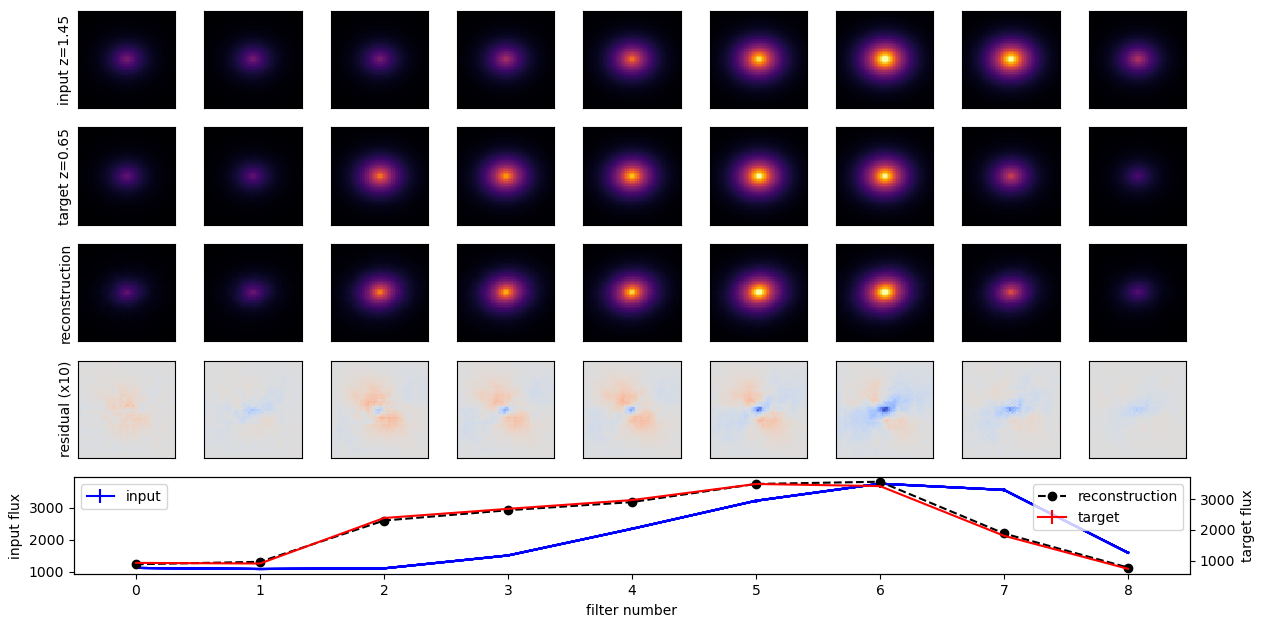
\includegraphics[width=\columnwidth]{Figures/standard-high-low.png}
        \caption{De-redshifting a simple galaxy image with no observational effects applied. Residuals are minimal and the reconstruction SED falls within the range of error for the target SED in all filters.}
        \label{fig:standard-high-low}
    \end{subfigure}
    
    \begin{subfigure}[b]{2\columnwidth}
        \centering
	    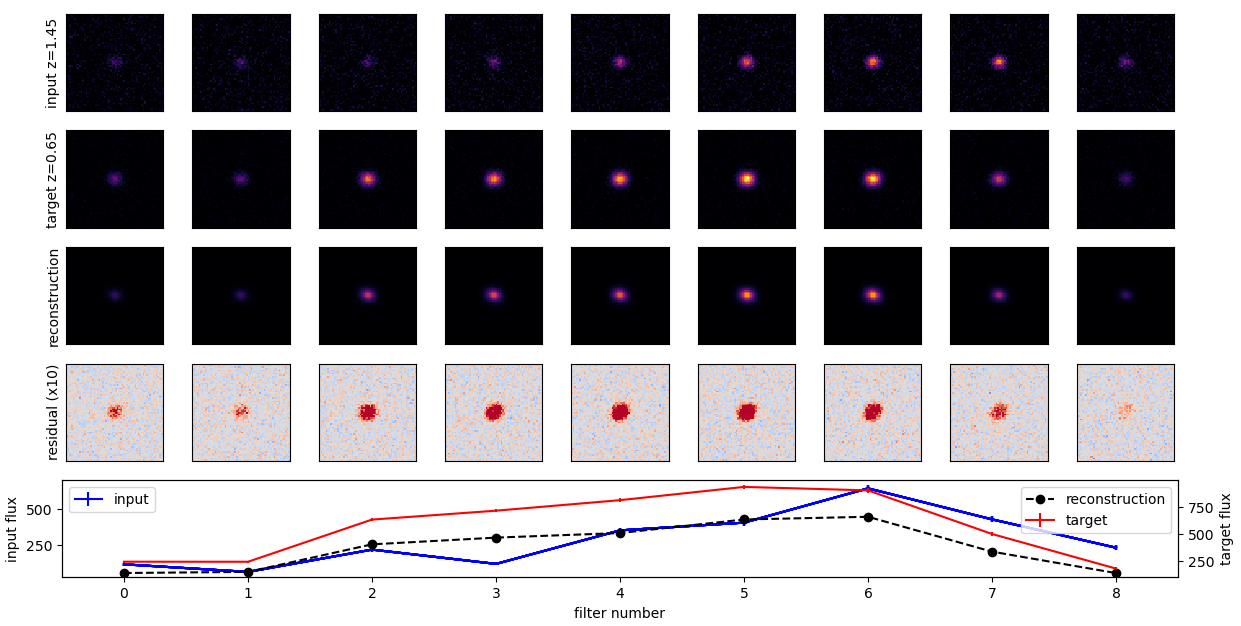
\includegraphics[width=\columnwidth]{Figures/noisy-high-low.png}
        \caption{De-redshifting a simple galaxy image with observational effects applied. Residuals are high due to the random noise within the image and the reconstruction SED does not match up with the target SED.}
        \label{fig:noisy-high-low}
    \end{subfigure}
    
    \caption{This galaxy has a high input redshift of 1.45 and a low target redshift of 0.65. The first row is the input redshift and the second row is the target redshift. The third row is the image reconstructions that the trained model has produced with the fourth row showing the residuals between the target and reconstructions. The plot on the fifth row shows the SED for the input, target and reconstruction images. The input and target SEDs have error bars correlating to the number of Poisson errors on each count.}
    \label{fig:simple galaxy results plots de-redshifting}

\end{figure*}

From what we learned with our tests on the original sample set, we recognised there was no need to run every test on this new sample. We know that the network particularly struggles to reconstruct noise. So, on the topic of increasing redshift, we tested how well the network can artificially increase the complex galaxies redshift, as well as removing noise. The reconstructions successfully remove the noise from the input galaxy. The residuals are minimal, but are noticeable. These residuals arise from differences in surface brightness between the target and reconstruction galaxy. The distribution of surface brightness is not perfect in the reconstruction. Generally, we found that the central bulge was brighter in the reconstruction and the surrounding disk was dimmer, when compared with the target. The residuals seen in Figure \ref{fig:complex-noisy-low-high} support this observation.

\begin{figure*}

    \begin{subfigure}[b]{2\columnwidth}
        \centering
	    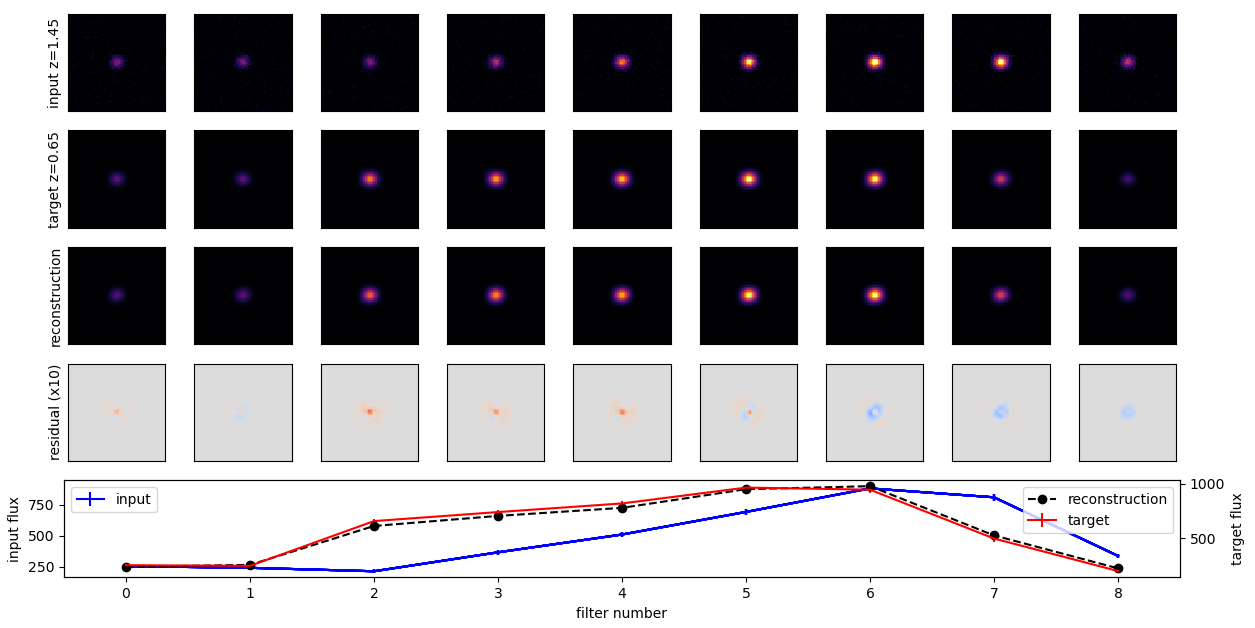
\includegraphics[width=\columnwidth]{Figures/noisy-high-noiseless-low.png}
        \caption{De-redshifting and de-noising a simple galaxy image. Residuals are minimal and the reconstruction and target SEDs match extremely well.}
        \label{fig:noisy-high-noiseless-low}
    \end{subfigure}
    
    \begin{subfigure}[b]{2\columnwidth}
        \centering
	    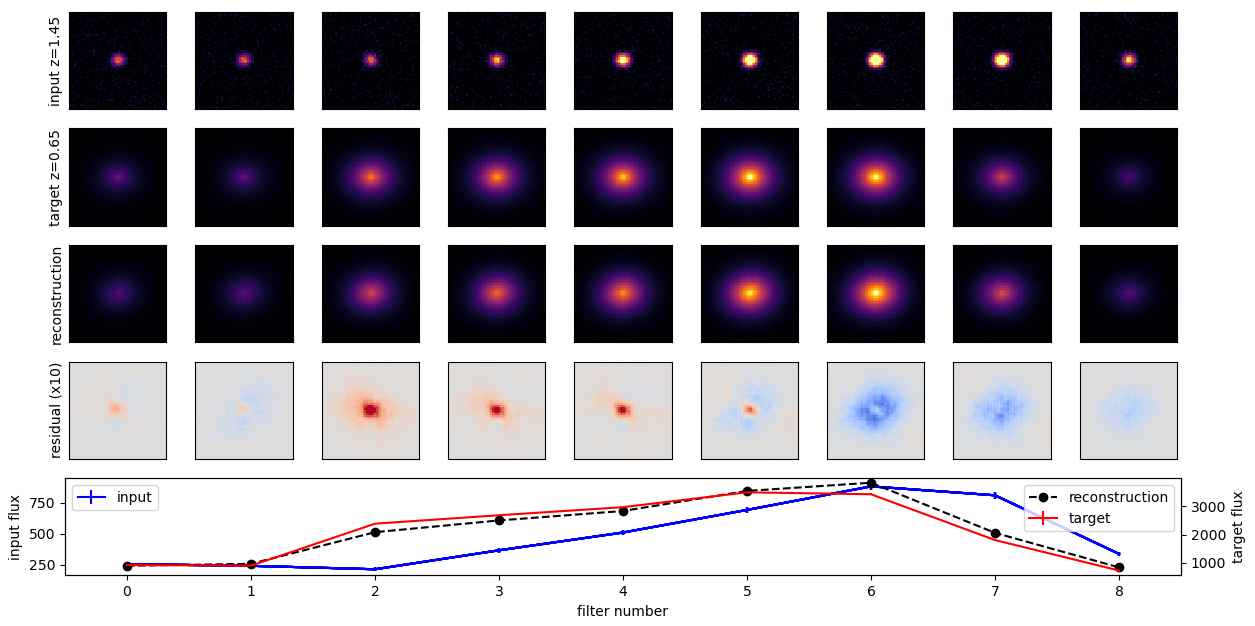
\includegraphics[width=\columnwidth]{Figures/noisy-high-standard-low.png}
        \caption{De-redshifting, de-noising and de-convolution applied to a simple galaxy image. Residuals are higher, however the reconstruction SED still falls within the margin of error of the target SED for nearly all filters.}
        \label{fig:noisy-high-standard-low}
    \end{subfigure}
    
    \caption{This galaxy has a high input redshift of 1.45 and a low target redshift of 0.65. The first row is the input redshift and the second row is the target redshift. The third row is the image reconstructions that the trained model has produced, with the fourth row showing the residuals between the target and reconstructions. The plot on the fifth row shows the SEDs for the input, target and reconstruction images. The input and target SEDs have error bars correlating to the number of Poisson errors on each count. }
    \label{fig:simple galaxy results plots de-noise}

\end{figure*}

\subsection{Decreasing Redshift} \label{sec:decreasing-redshift}
\subsubsection{Standard Galaxies} \label{sec:standard-test2}
The alternative test with the same sample of galaxies was to give the network a galaxy at a higher redshift and train it to reconstruct the galaxy at a lower redshift. The reconstructions in this instance were also very accurate with minimal residual. The network has no problem when learning to add or remove artificial dimming from the galaxies. Figure \ref{fig:standard-high-low} is one example of how well the network can reconstruct galaxies at a lower redshift. From this test alone, we can see that the network does not perform differently while redshifting or de-redshifting a galaxy.

\begin{figure*}

    \begin{subfigure}[b]{2\columnwidth}
        \centering
	    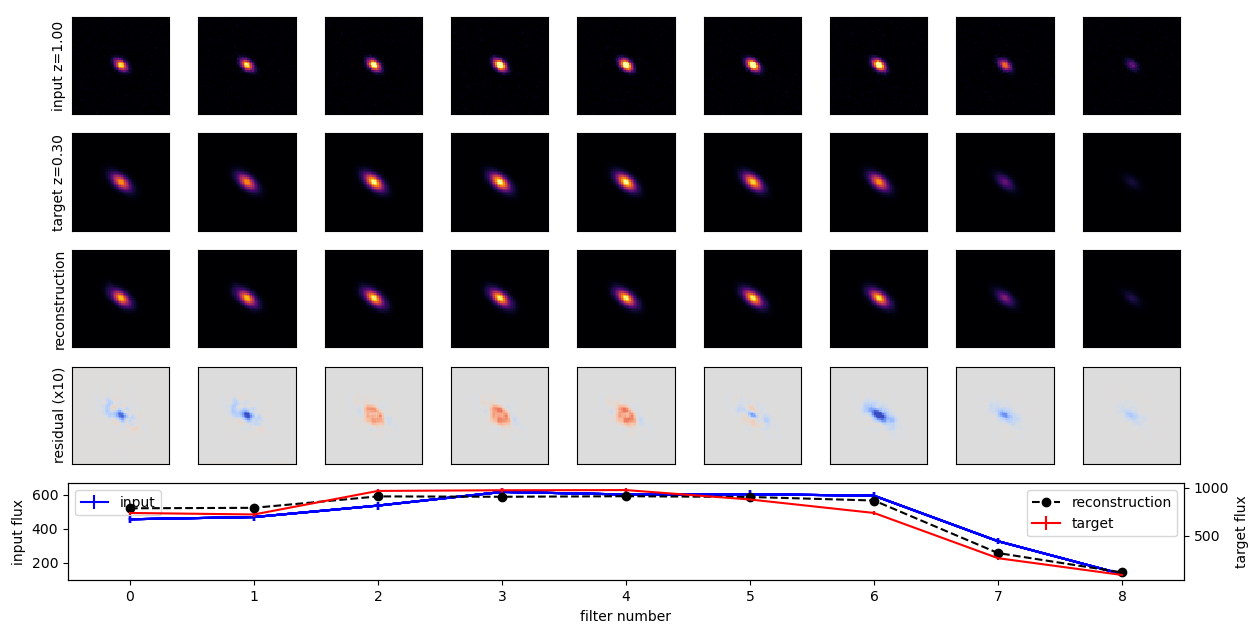
\includegraphics[width=\columnwidth]{Figures/bd-noisy-high-noiseless-low.png}
        \caption{De-redshifting and de-noising a complex galaxy image. Residuals are fairly minimal and the reconstruction SED falls within the margin of error of the target SED for nearly all filters.}
        \label{fig:complex-noisy-high-noiseless-low}
    \end{subfigure}
    
    \begin{subfigure}[b]{2\columnwidth}
        \centering
	    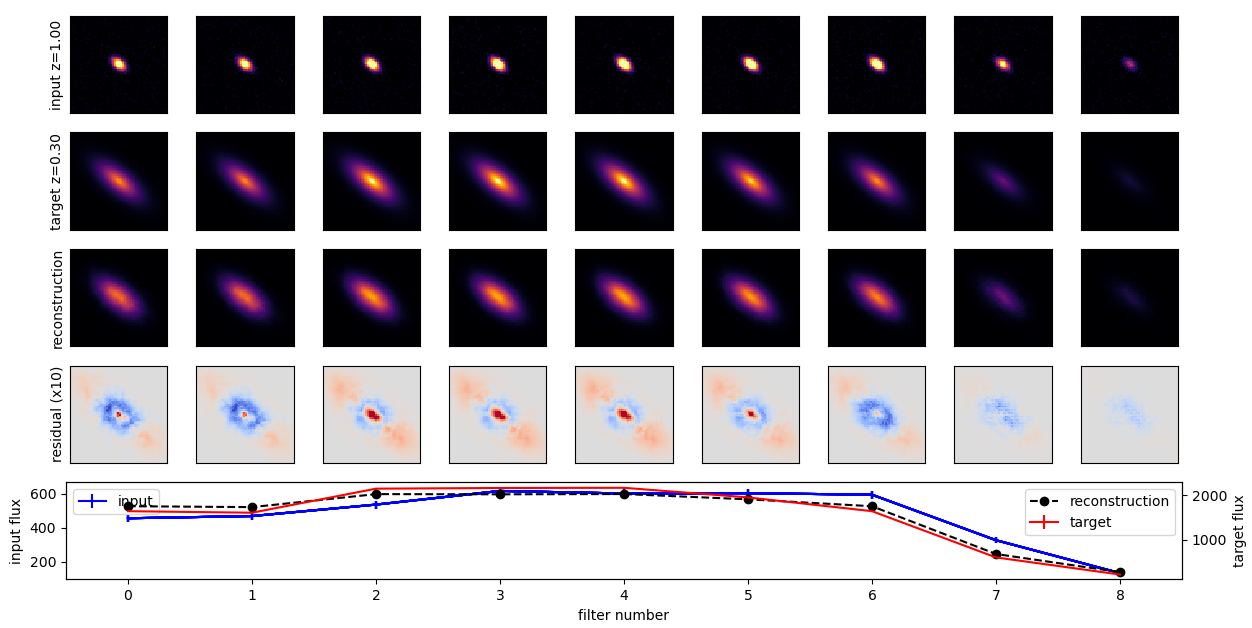
\includegraphics[width=\columnwidth]{Figures/bd-noisy-high-standard-low.png}
        \caption{De-redshifting, de-noising and de-convolution applied to a complex galaxy image. Residuals are higher, however the reconstruction SED falls within the margin of error of the target SED for all filters and error per pixel was calculated to be only 10\%}
        \label{fig:complex-noisy-high-standard-low}
    \end{subfigure}
    
    \caption{This complex galaxy has a high input redshift of 1.00 and a low target redshift of 0.30. The first row is the input redshift and the second row is the target redshift. The third row is the image reconstructions that the trained model has produced, with the fourth row showing the residuals between the target and reconstructions. The plot on the fifth row shows the SED for the input, target and reconstruction images. The input and target SEDs have error bars correlating to the number of Poisson errors on each count.}
    \label{fig:complex galaxy results plots de-noise}

\end{figure*}

\subsubsection{Observed Galaxies} \label{sec:observed-test2}
The network performs in a similar way reconstructing a noisy lower redshift galaxy given the galaxy at a higher redshift. The reconstructions are also missing noise. The severity of the residual noise depends on how noisy the target it. For lower redshift galaxies ($z \leq 1$) the noise is generally low, which in turn leaves less residual. Figure \ref{fig:noisy-high-low} includes a galaxy that is fairly noisy, which is reflected in the residuals. Nonetheless, the reconstructions are accurate in terms of shape and size. The network not being able to reconstruct noise is not a bad result, however as it means the network is effectively de-noising the input galaxies despite not being trained for this purpose. This is very useful for situations where you want to study properties of galaxies independent of redshifting effects, such as shot and background noise.

\subsubsection{De-noising Galaxies} \label{sec:de-noise-test}
With our full tool-set, we have the ability to alter how we generate and process our galaxy images. This allows us to take our tests in a more practical direction. We can artificially add and remove noise from our galaxies and intentionally train the network to not reconstruct noise. For this test we had the network reconstruct an observed galaxy without the background and shot noise applied, given the input galaxy at a higher redshift with the noise applied. This time we were intentionally wanting the network to not reconstruct noise, thus de-noising the input galaxy. Figure \ref{fig:noisy-high-noiseless-low} gives an example of the networks ability to artificially remove noise from the galaxy. The residuals are small and comparable to those mentioned in Section \ref{sec:standard-test}.

\subsubsection{De-noising and De-convolving Galaxies} \label{sec:de-noise-convolve}
To further test the idea of artificially de-redshifting galaxies, we trained the network to not reconstruct the PSF, as well as the background and shot noise. The result of this process is the ability to take a galaxy at a higher redshift and reconstruct it at a lower redshift, while also removing the redshifting effects. The network performs reasonably when asked to reconstruct a target galaxy without the mentioned redshifting effects, as seen in Figure \ref{fig:noisy-high-standard-low}. The residuals show more discrepancy than some of the other tests, however the reconstruction and target match very closely. Just like in Section \ref{sec:de-noise-test}, the network has no trouble removing noise. Reversing the convolution process seems more challenging, which is reflected in the residuals. The shape and size are reconstructed well, as expected. However, we see that the distribution of surface brightness is not perfectly matched. This is reflected in the comparison of target and reconstruction SED at the bottom of Figure \ref{fig:noisy-high-standard-low}.

\subsubsection{Complex Galaxies} \label{sec:complex-de-redshifting}
We ran 2 different tests in order to test the networks ability to de-redshift a complex galaxy at various levels. Firstly, we had the network reconstruct our set of complex galaxies at a lower redshift without any noise. The network was able to successfully remove the noise from the input galaxy and reconstruct the galaxies shape reasonably well. Similarly to what we saw in Section \ref{sec:complex-redshifting}, the network is struggling to reconstruct the distribution of surface brightness correctly. Parts of the galaxy are brighter than they should be, and some are fainter. This discrepancy is not significant. The bottom row of Figure \ref{fig:complex-noisy-high-noiseless-low} shows the difference in flux between the target and reconstructed galaxy. 

Finally, we had the network remove the noise and the PSF convolution. The difference between the reconstruction and target galaxy on average is more prominent than in the case of just removing noise which is to be expected. Nevertheless, when compared to the same test performed on the original galaxy set, the network performs just as well, and the percentage error pixel is only 10\%. The introduction of new shapes in the galaxy images has not effected the networks performance. As usual, we are seeing differences in surface brightness, rather than shape or size. Figure \ref{fig:complex-noisy-high-standard-low} shows the comparison of the target and reconstructed galaxy. The difference in SED, seen on the bottom row, is actually an improvement when compared with Figure \ref{fig:complex-noisy-high-noiseless-low}. The central bulge appears slightly dimmer in the reconstruction than it should be.

\section{Discussion}
\label{sec:discussion}

\subsection{Simulating Galaxies} \label{sec:simulate-discussion}
As mentioned in Section \ref{sec:simulate}, the shape of the galaxies generated were controlled by 3 varying parameters: the ellipticity, effective radius and rotation angle. Each of these parameters were randomly selected to a precision of 2 decimal places. This was a choice made to avoid unnecessary precision. It helped with improving processing times and did not lead to a noticeable change in the production of galaxy images.

After combining the SEDs with our S\'ersic galaxies, we had our galaxy set observed in 17 different filters for a range of redshifts. The range in filters was required to perform the redshifting, which corresponded to a shift in the galaxies SED. The more filters available to us in the given range (low to mid infrared), the more accurate the shift in SED. After some tests with applying observational effects (Section \ref{sec:observe}) and running the galaxies through the CVAE (Section \ref{sec:network}) we determined that we should reduce the number of filters used to reduce the size of our data set. This reduction was from 17 to 9 filters. This was a large step in improving the processing time and resources used when training the network. For the number of galaxies we were running through the network ($n = 10,000$) this improvement was necessary. However, with this change came an increase in the inaccuracy of the SED shift. With roughly half the number of data points in the filter range, the accuracy of the SED shift roughly halves.

The ability to generate more complex images of galaxies gave us a good opportunity to further test the network. In Section \ref{sec:complex} we outline two different methods of varying the sample of galaxies we produce. We were able to test the network on the two component galaxies (bulge and disk) in Section \ref{sec:complex-redshifting} and \ref{sec:complex-redshifting}. In the second variation to the sample we introduced asymmetry. Unfortunately, we did not have chance to run any tests with this sample. However, based on the way our network was able to reconstruct shapes, we estimate that the network would have no problem with de-redshifting asymmetric galaxy images. The opportunity to test our network on asymmetric galaxies would have provided more insight into the networks capability with real galaxy images.

On the topic of realistic galaxies, adding more galactic features to our images would improve the diversity of our sample and allow us to learn more about the networks capability. Some of the features we could have included are spiral arms, bar shaped central bulges and background objects (such as other stars or galaxies). If the network was used to process real galaxies images, we would want the training set of simulated galaxies to resemble the real set as best as possible. 

\subsection{Observational Effects} \label{sec:observational-discussion}
Each observational effect was applied to the images in a series of dedicated functions, as described in Section \ref{sec:observe}. The code was designed this way to allow the addition and removal of different observational effects when running various tests with the neural network.

As mentioned in Section \ref{sec:rebinning}, whilst the size of the galaxy needed correcting, we wanted the overall image size to remain the same for running through the network. The zoom function was used to rescale the images, however this function changed the image size as a whole. This proved difficult when transforming a galaxy from low to high redshift as the size of the images would decrease. As a result, when performing these transformations there was insufficient data for the function to fill around the edge of the image. Initial attempts to fix this issue were made by padding the edges of the images with zeroes to fill up to the original 60 by 60 pixel size. This was not successful nor realistic. To instead overcome the issue, broadcasting and interpolation techniques were applied (see Section \ref{sec:rebinning}). This method interpolated the pixels from the original image grid to a rescaled grid with the same number of pixels. Though this method was successful, the interpolated data is only an estimation of realistic values and not true values themselves. If we had more time, a more suited solution to this issue would be to initially create the simulated images at the correct size using a method of image resampling \citep{Devillard2000}. This would instead be performed in the galaxy simulation stage. Oversampling is one such method that could be implemented to achieve higher resolution images with lower SNR. 

The last observational effects applied were shot noise and background noise. A Poisson distribution and Gaussian distribution were applied respectively to model these types of noise. Whilst this produced reasonable recreations of the noise you might see when observing real galaxies, the network struggled to produce reconstructions with realistic noise from the simulated galaxy images. This can be seen in Figure \ref{fig:noisy-low-high} where the residual images are dominated by noise. The galaxies themselves were reconstructed well, however the noise was not being learned by the network. Given more time, the simulation and addition of noise could be improved upon. In the FERENGI paper, background noise is added from real data instead of random distributions (see Section 4 of \citet{Barden2008}). The galaxies are added to blank sky taken from actual observations, leading to better representations of empty sky regions. This method could be used in place of the Gaussian distribution in the future for more realistic noise within our simulated images. Background noise can often show correlations as a result of faint astronomical objects or image processing effects. Using actual data to fill the background would therefore be the most direct and accurate way of including these correlations. This step could be applied afterward, rather than before running through the network. Adding noise in this order would reduce the difference seen within the residuals as the network no longer needs to learn noise.

\subsection{Neural Network} \label{sec:NN-discussion}
From Figures \ref{fig:standard-low-high},  \ref{fig:standard-high-low} and \ref{fig:complex-standard-low-high} it can be seen that the training the CVAE with 10,000 images worked very well for creating models that were able to accurately redshift, de-redshift and as a result simulate the artificial addition and subtraction of dimming. However, it can be noted that whilst residuals were fairly minimal for both the redshifting and de-redshifting models, they were slightly higher on that of the de-redshifting. This is to be expected as this is a harder process for the network to learn since there is a certain ambiguity over what the galaxy actually looks like, since the network is essentially being given low resolution information and being told to make it high resolution. There also appeared to be no noticeable difference in the results between the same experiments run on both simple and complex galaxies. This is promising and a good indicator that the network is able to learn shape well, as it was able to still effectively learn the appearance of a galaxy despite the addition of more complex features.

The process of learning to redshift observed galaxies, as seen in Section \ref{sec:observed-test}, is a lot harder for the network to learn and as a result was not as much of a successful experiment. The addition of the shot noise and background noise in particular means that the residuals are lot higher than those in the ‘standard' galaxy experiments as seen in Figures \ref{fig:noisy-low-high} and \ref{fig:noisy-high-low}. This is because the noise in each galaxy image is random, meaning that the CVAE is not able to learn a pattern so that it can accurately generate an observed galaxy image of its own. Nevertheless, the models that were created after training on these `noisy' images were able to learn the galaxy shapes, size, and brightness fairly well, suggesting that the network can model the galaxies fairly accurately even with the addition of observational effects. Models trained on noiseless data were also then tested with these noisy input images to see if they could effectively reconstruct the galaxies. However, it was found that the images were actually worse than the models trained on the `noisy' data. This is likely due to the introduction of individual normalisation of the galaxies, which was a necessary feature as before this was introduced the network was giving losses of NaN. This normalisation value is likely different for both the noisy and noiseless galaxy images, thus when a model trained on one type of data is then applied to the other there is a conflict, suggesting that consistency between noisy and non-noisy image normalisation is what is needed. Due to time constraints of this project, this solution was not able to be tested, however it is likely that the best way for the CVAE to reconstruct `noisy' galaxy images is to use a model that was trained on noiseless images since this appears to have better reconstruction quality for galaxy features.

Whilst generating a noisy image of a galaxy was a good test for the network it has less extensive real life applications. A more useful technique would be the ability to de-noise galaxy images so that their characteristics and shapes can be better identified. Thus, the CVAE was trained to perform this technique as described in Section \ref{sec:de-noise-test}. This was very successful with residuals being minimal and noise within the reconstructions being low, as can be seen from Figure \ref{fig:noisy-high-noiseless-low} and \ref{fig:complex-noisy-high-noiseless-low}. The process of then taking this a step further by introducing de-convolution in addition to the de-redshifting and de-noising was the next logical step. This again had fairly good results, as seen in Figure \ref{fig:noisy-high-standard-low} and \ref{fig:complex-noisy-high-standard-low}. The residuals are noticeably higher, however when quantifying the percentage error per pixel it was found that the worst residuals had an error of only 10\%. A higher percentage of error is to be expected for this experiment in particular as removing multiple observational effects is a more complex process. Training for longer or with a larger amount of images might be more advisable for this model in particular. Nevertheless, these initial results are extremely good, and show promising capabilities for application to observed galaxy images.

Though the residuals were higher in some of these experiments than others there seems to be a general pattern to them. The residuals tend to be due to a difference in surface brightness between the target and reconstruction. This could be a result of the network overfitting, which has several solutions, such as the addition of a Gaussian noise layer in the encoder that was added, so that a different pattern of noise is added within each layer, making it harder for the network to learn the galaxy images ‘too well', essentially regularising the model. A standard deviation of 0.2 was selected for the Gaussian noise layer that was included, this value is quite low so the difference it is making is likely not effective as it could be. To select a better value identical runs would need to be made with different noise levels, however due to time constraints within this project this was not able to be investigated.

Another approach that could be taken, but was again not able to be tested within the time constraints of this project, was the addition of a dropout layer which randomly cuts a percentage of the connection from one layer to the next in the encoder and decoder forcing the network to learn a superposition of the model. These systematic residuals could potentially be quantified by building uncertainties into the network, see \citet{Perreault2017, Pearson2021}, through the introduction of the dropout layer. Currently the network has problems discerning from a high redshift input image whether the galaxy is large and compacted or small and uncompacted, as it attempts to construct a low redshift target image. The inclusion of a dropout layer would allow for the network to produce a variety of images as to what the galaxy could have looked like, which would allow for a better reconstructions on surface brightness concentration. Error bars could also then be added to the reconstruction line in the SED plots for the galaxy images, as there would then be quantifiable uncertainties.

Another source for these errors could be because of bias in the simulated galaxies training sample as mentioned in Section \ref{sec:simulate-discussion}. If there is a lower percentage of elliptical galaxies than round, then the network will find these harder to reproduce. This issue could be overcome by using a larger sample size, however the size used for this project (10,000 galaxies) was chosen as the limit due to RAM capacities. Alternatively, training for longer could also be beneficial which is why the patience on the callback was temporarily increased to 25 but it was found that this did not have much of an effect. The risk of training for too long also comes with its own negative effects, as this would lead to the loss function reaching its minimum value which also causes overfitting.

Time constraints within this project also meant that hyperparameter optimisation was not able to performed such as in \citet{Bergestra2011, Hutter2011}. Meaning that a variety of values for as many hyperparameters as possible (i.e. beta, kernel size, number of latent dimensions) were not able to be explored. Whilst the CVAE works extremely well without this exploration optimizing these values would likely improve the remaining residuals. 

Lastly whilst the error of 10\% is extremely good, it is still fairly approximate. Due to time constraints the process was not able to repeated and regularised for all filters in all experiments. As previously mentioned however, the experiment for which the error of 10\% is attributed to is the most complex one that was run (see Section \ref{sec:de-noise-convolve}), so therefore gives an accurate idea as to the capabilities of the precision of the network. The circle within which to average the errors that was selected as shown in Figure \ref{fig:errorplot}, was chosen to have a centre that was the centre of the galaxy image and the radius was based on the encompassment of the residuals in the central area. The pixel errors across the whole image could not be averaged, due to the corners of the image within which no galaxy was present, as can be seen in the top right and bottom left corners of Figure \ref{fig:errorplot}. This is because these regions tend to not only be typically noisier (when noisy images are being used) but also have very low fluxes. Meaning that when the reconstruction is divided by the target image, it is divided by a very small number which then gives a very large percentage error and consequentially skews the results. A better way to standardise the errors would be to create a circle the same size as the half light radius of the galaxy within which pixel errors could then be averaged, but due to time constraints this was also not able to be tested.

\section{Conclusion}
In this study we trained a neural network to reconstruct simulated galaxy images with added or removed redshifting effects. These effects are outlined in Section \ref{sec:simulate} and \ref{sec:observe}. Our method of simulating galaxies gave us a variety shape, size and surface brightness. With the addition of complex simulated galaxies (Section \ref{sec:complex}), we had a diverse sample set to train and test the network with. By applying observational effects independently, we were able to perform separate tests with or without certain effects. This helped with identifying the networks strengths and weaknesses for a sample of our size ($n=10,000$).

The models created by the CVAE work extremely well in both redshifting and de-redshifting simple and complex simulated galaxy images. The addition of the artificial effects makes it harder for the network to perform these same processes due to the addition of the random noise but it is still able to generally reconstruct the galaxy's shape and size. In the training of the CVAE to perform de-noising and de-convolution of galaxy images it works extremely well with minimal residuals and a maximum percentage error per pixel of 10\%. The application of these techniques to future projects could have wide ranging implications, enabling us to more clearly see and compare high redshift galaxies without the observational effects that currently obscure them.

Sources of error were minimal because the base of the project was computational, however resulting residuals can be attributed to overfitting, a bias training sample or a training sample that is too small. Hyperparameter optimisation could also improve remaining residuals through the exploration of a variety of values for parameters such as the number of latent dimensions, kernel size, and beta. The introduction of a dropout layer into the network would allow uncertainties on the reconstruction images to be more readily quantified, and averaging these pixel errors across the half light radius of the galaxies would allow for better standardisation. 

%%%%%%%%%%%%%%%%%%%%%%%%%%%%%%%%%%%%%%%%%%%%%%%%%%
%\section*{Data Availability}

 
%The inclusion of a Data Availability Statement is a requirement for articles published in MNRAS. Data Availability Statements provide a standardised format for readers to understand the availability of data underlying the research results described in the article. The statement may refer to original data generated in the course of the study or to third-party data analysed in the article. The statement should describe and provide means of access, where possible, by linking to the data or providing the required accession numbers for the relevant databases or DOIs.




%%%%%%%%%%%%%%%%%%%% REFERENCES %%%%%%%%%%%%%%%%%%

% The best way to enter references is to use BibTeX:

\bibliographystyle{mnras}
\bibliography{references} % if your bibtex file is called example.bib


% Alternatively you could enter them by hand, like this:
% This method is tedious and prone to error if you have lots of references
%\begin{thebibliography}{99}
%\bibitem[\protect\citeauthoryear{Author}{2012}]{Author2012}
%Author A.~N., 2013, Journal of Improbable Astronomy, 1, 1
%\bibitem[\protect\citeauthoryear{Others}{2013}]{Others2013}
%Others S., 2012, Journal of Interesting Stuff, 17, 198
%\end{thebibliography}

%%%%%%%%%%%%%%%%%%%%%%%%%%%%%%%%%%%%%%%%%%%%%%%%%%

%%%%%%%%%%%%%%%%% APPENDICES %%%%%%%%%%%%%%%%%%%%%

%\appendix

%\section{Some extra material}

%If you want to present additional material which would interrupt the flow of the main paper,
%it can be placed in an Appendix which appears after the list of references.

%%%%%%%%%%%%%%%%%%%%%%%%%%%%%%%%%%%%%%%%%%%%%%%%%%


% Don't change these lines
%\bsp	% typesetting comment
\label{lastpage}
\end{document}

% End of mnras_template.tex
